\chapter{Experiments and results} \label{sec:experiments-and-results}
This chapter provides a detailed account of the experimental methodology and results obtained to establish a baseline for NeRFs trained on synthetic data captured from the CARLA simulator. The defined baseline is then utilized to conduct further experiments investigating the impact of various settings and methods for training NeRFs, including pre-processing, different NeRF-models, and camera optimization. Furthermore, the experiments’ insights are applied to evaluate the proposed pipeline’s transferability from synthetic to real data.

The results obtained from the experiments are evaluated both quantitatively, using the metrics discussed in \autoref{sec:evaluating-nerfs}, and qualitatively. The included qualitative results are frames extracted from video renders of the respective NeRFs. Although the frames convey important results, the video renders provide a much clearer understanding of correspondences between frames, potential artifacts, learned geometry, and other relevant information. To showcase these results, a companion page is available where different renders from this chapter's experiments can be browsed and compared.

Quantitative results are highlighted in the tables, with \ulcolor[green]{green} signifying the best results, and \ulcolor[red]{red} indicating the worst. \ulcolor[blue]{Blue} is employed to denote a configuration selected for subsequent experiments.

\vspace{2mm} %5mm vertical space
\noindent \textbf{\href{https://absorbing-peace-5f6.notion.site/NeRF-Renders-Master-thesis-34ff125e2200406588f002b36eeaacef}{Link to companion page with video renders}}


\newpage
\section{Experiment 1: Defining a Baseline}

To facilitate comparison between experiments, it is crucial to establish a baseline. However, no existing baselines for NeRF models trained on synthetic data captured in CARLA currently exist. Therefore, this study defined a baseline by optimizing settings across various categories in CARLA, including camera setup, capacity, camera settings, vehicle speed, and number of frames. Both a quantitative and qualitative assessment was conducted for the results of each experiment. Based on the assessment, one of the configurations was selected and kept for further experiments.

By establishing this baseline, it can be used as a reference point for improving both the data capture and NeRF models on synthetic data. The metrics used to evaluate the baseline (\acrshort{psnr}, \acrshort{ssim}, and \acrshort{lpips}) are widely used in NeRF research, ensuring the comparability of results with future experiments and research.

The CARLA configurations held constant for the respective experiments are depicted in \autoref{tab:combined-baseline-constant-parameters}.

\begin{table}[ht]
\centering
\setlength{\tabcolsep}{6pt}
\renewcommand{\arraystretch}{1.5}
\begin{tabular}{c | c c c c c}
% \multicolumn{}{c}{\textbf{Experiment setup - constant variables}} \\
\hline
Experiment & Camera setup & Distance & Image freq. & Image res. & Speed \\
\hline
\hyperref[sec:exp-camera-setup]{1.1} & $-$                                                 & 125m                      & 3     & $600 \times 450$  & 100\% \\
\hyperref[sec:exp-capacity]{1.2} &\cellcolor{blue} $[-10^{\circ}, 10^{\circ}]$ yaw     & $-$                       & 3     & $600 \times 450$  & 100\% \\
\hyperref[sec:exp-number-of-frames]{1.3} &\cellcolor{blue} $[-10^{\circ}, 10^{\circ}]$ yaw     &\cellcolor{blue} 4 turns   & $-$   & $600 \times 450$  & 100\% \\
\hyperref[sec:exp-image-resolution]{1.4} &\cellcolor{blue} $[-10^{\circ}, 10^{\circ}]$ yaw     &\cellcolor{blue} 4 turns   &\cellcolor{blue} 2     & $-$               & 100\% \\
\hyperref[sec:exp-speed]{1.5} &\cellcolor{blue} $[-10^{\circ}, 10^{\circ}]$ yaw     &\cellcolor{blue} 4 turns   &\cellcolor{blue} 2     &\cellcolor{blue} $400 \times 300$  & $-$ \\
\hyperref[sec:exp-combined-baseline]{1.6} &\cellcolor{blue} $[-10^{\circ}, 10^{\circ}]$ yaw     &\cellcolor{blue} 4 turns   &\cellcolor{blue} 2     &\cellcolor{blue} $400 \times 300$  &\cellcolor{blue} 50\% \\
\hline
\end{tabular}
\caption[Constant parameters for the experiments conducted to define a baseline]{Overview of the configurations that were kept constant for each experiment conducted to define the baseline. The configurations that were selected to be part of the baseline data capture configuration, based on the results from the experiments, are highlighted in \ulcolor[blue]{blue}}
\label{tab:combined-baseline-constant-parameters}
\end{table}









\subsection{Experiment 1.1: Camera Setup} \label{sec:exp-camera-setup}
The CARLA simulator provides a convenient way to attach multiple cameras with varying settings to a vehicle. To optimize the performance of NeRFs on RGB images, a series of experiments were conducted to determine the optimal camera setup based on the three metrics: \acrshort{psnr}, \acrshort{ssim}, \acrshort{lpips}. All cameras were positioned at the same base translation, at the roof of the ego vehicle approximately 3 meters above ground level. While this camera placement may be considered unrealistically elevated, it facilitates an unobstructed capture of the scene without interference from the ego vehicle. The camera setups tested in this study were:

% TODO: Add figure with the camera setups?
\begin{itemize}
    \item Single forward-facing camera.
    \item Two forward-facing cameras, with a counterrotated yaw.
    \item Three cameras, one with zero yaw and two with counterrotated yaw.
\end{itemize}

\begin{table}[ht]
\centering
\setlength{\tabcolsep}{6pt}
\renewcommand{\arraystretch}{1.5}
\begin{tabular}{l | C{2.2} C{1.3} C{1.3}}
\hline
\textbf{Description} & \textbf{PSNR $\uparrow$} & \textbf{SSIM $\uparrow$} & \textbf{LPIPS $\downarrow$} \\
\hline
Single camera, $[0^{\circ}]$ yaw & 22.764567 & 0.74230 & 0.150325 \\
\cellcolor{blue}Two cameras, $[-10^{\circ}, 10^{\circ}]$ yaw & 23.900909 & \cellcolor{green} 0.782013 & \cellcolor{green} 0.135604 \\
Two cameras, $[-30^{\circ}, 30^{\circ}]$ yaw & \cellcolor{red} 23.235004 & 0.755689 & 0.155470 \\
Two cameras, $[-50^{\circ}, 50^{\circ}]$ yaw & 23.732924 & \cellcolor{red} 0.739246 & 0.174111 \\
Two cameras, $[-70^{\circ}, 70^{\circ}]$ yaw & \cellcolor{green} 24.318214 & 0.739551 & 0.172868 \\
Three cameras,  $[-50^{\circ}, 0^{\circ}, 50^{\circ}]$ yaw & 23.785522 & 0.763684 & 0.165152 \\
Three cameras,  $[-70^{\circ}, 0^{\circ}, 70^{\circ}]$ yaw & 23.684502 & 0.754842 & \cellcolor{red} 0.176524 \\
\hline
\end{tabular}
\caption[Results for experiment 1.1: Camera setup]{Comparison of different camera setups' impact on the NeRF's performance.}
\label{tab:exp_camera_setup}
\end{table}

\begin{comment}
\vspace{0.5cm}

\setlength{\tabcolsep}{12pt}
\renewcommand{\arraystretch}{1.2}
\begin{tabular}{l l}
\multicolumn{2}{c}{\textbf{Experiment setup - constant variables}} \\
\hline
Parameter & Value \\
\hline
Distance  & 125 meters \\
Image resolution &  $600 \times 450$ \\
Ticks per image & 3 \\
Speed & 100\% (default: 30km/h) \\
\hline
\end{tabular}
\caption[Constant parameters for experiment 1.1]{Overview of the values of the parameters that remained constant across the experiments' runs.}
\label{tab:camera-setup-stable-variables}
\end{comment}



% Overall, the results suggest that a camera setup with two cameras at -10$^{\circ}$ and 10$^{\circ}$ yaw produces the highest quality images, while setups with more than two cameras do not necessarily result in significantly higher quality images
From \autoref{tab:exp_camera_setup}, we can see that the camera setups produce relatively similar results across the three metrics, with only small differences between them. The camera setup with two cameras at -70$^{\circ}$ and 70$^{\circ}$ yaw achieves the highest \acrshort{psnr} score, indicating that it produces the most accurate images. On the other hand, the configuration with two cameras at $-10^{\circ}$ and $10^{\circ}$ yaw achieves the highest \acrshort{ssim} and lowest \acrshort{lpips} scores, indicating that it produces the most visually similar and perceptually pleasing images. Due to the configuration's high \acrshort{ssim} and low \acrshort{lpips}, it was chosen as the camera setup baseline for further experiments.

% ADD THIS TO THE DISCUSSION-PART
% The reason for -10 and 10 being the best performing: Trained more on the images it was later evaluated on, since the evaluation images are 10% of the original training data.










\subsection{Experiment 1.2: Capacity} \label{sec:exp-capacity}
As discussed in \autoref{sec:block-nerf} and \autoref{sec:method-block-nerf}, the capacity of a NeRF is limited. In order to quantitatively assess this capacity, an experiment was designed involving five increasingly longer routes for a CARLA vehicle to capture data. The routes' length ranged from 50m to approximately 450m, as depicted in Figure \ref{fig:capacity-overview}. The longest route corresponds to a full lap around the block.


\begin{table}[ht]
\centering
\setlength{\tabcolsep}{6pt}
\renewcommand{\arraystretch}{1.5}
\begin{tabular}{l | C{2.2} C{1.3} C{1.3}}
\hline
\textbf{Description} & \textbf{PSNR $\uparrow$} & \textbf{SSIM $\uparrow$} & \textbf{LPIPS $\downarrow$} \\
\hline
50 meters & 23.541059 & \cellcolor{green} 0.773228 & \cellcolor{green} 0.108571 \\
100 meters & 23.594120 & 0.763471 & 0.141350 \\
2 turns & \cellcolor{green} 23.599499 & 0.756889 & 0.181586 \\
3 turns & 22.634428 & 0.719888 & 0.210503 \\
\cellcolor{blue}4 turns & \cellcolor{red} 22.500532 & \cellcolor{red} 0.695553 & \cellcolor{red} 0.240513 \\
\hline
\end{tabular}
\caption[Results for experiment 1.2: Capacity.]{Comparison of different segment lengths' impact on the NeRF's performance.}
\label{tab:exp_capacity-2}

\end{table}

\begin{comment}
\vspace{0.5cm}

\setlength{\tabcolsep}{12pt}
\renewcommand{\arraystretch}{1.2}

\begin{tabular}{l l}
\multicolumn{2}{c}{\textbf{Experiment setup - constant variables}} \\
\hline
Parameter & Value \\
\hline
\cellcolor{blue}Camera setup &\cellcolor{blue}Two cameras, $[-10^{\circ}, 10^{\circ}]$ yaw \\
Image resolution &  $600 \times 450$ \\
Ticks per image & 3 \\
Speed & 100\% (default: 30km/h) \\
\hline
\end{tabular}
\caption[Constant parameters for experiment 1.2.]{Overview of the values of the parameters that remained constant across the experiments' runs.}
\label{tab:exp-capacity-stable-variables}
\end{comment}


\begin{figure}[!h]
    \centering
    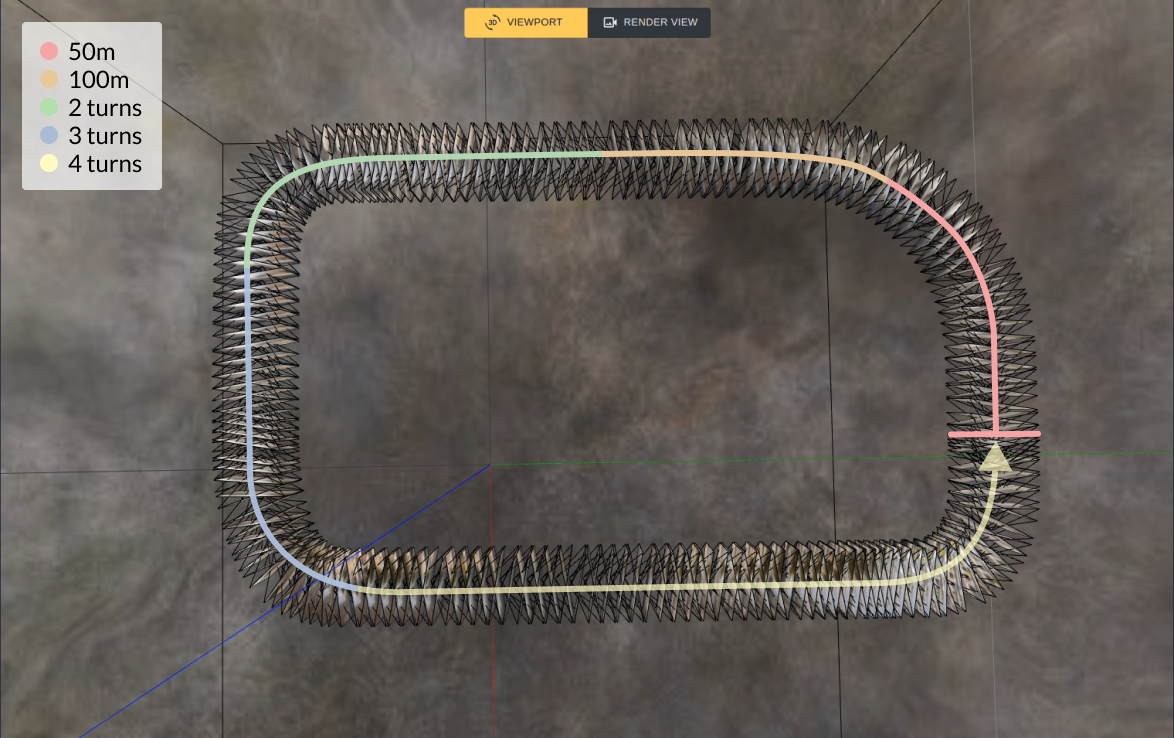
\includegraphics[width=1.0\textwidth]{figures/capacity-overview.png}
    \caption[Overview of the segments used in Experiment 1.2.]{Overview of the increasingly longer routes used to capture data in CARLA, during experiment 1.2.}
    \label{fig:capacity-overview}
\end{figure}

% Which configuration is included in the baseline, and briefly "why"?
The results show that the quality of the rendered images degrades as the segments’ length increases. The longest segment, the full lap around the block which includes four turns, achieves the worst results across all three metrics. Despite achieving the worst results, we selected the longest run as the baseline for further experiments. This is because conducting experiments on a full lap around the block provides a more realistic scenario for evaluating the performance of the NeRF on data captured by a vehicle. The full lap encompasses a variety of different scenes, including straight roads, curves, intersections, and varying lighting conditions. This diverse range of environments can help to test the NeRF’s ability to learn a varying scene and provide a more comprehensive evaluation of its performance.

% Things to discuss
%- The PSNR remains relatively constant across the segments, while the SSIM and LPIPS metrics show a clear downward trend.











\subsection{Experiment 1.3: Number of Frames} \label{sec:exp-number-of-frames}
%The number of input images used to train the NeRF should significantly affect its performance. 
A NeRF's dataset is comprised of images and corresponding camera poses. The size of this dataset determines the amount of information available for the NeRF to learn the underlying 3D scene structure and appearance. A larger dataset can provide more diverse and detailed information about the scene, which can help the NeRF to capture fine-grained details and generalize better to novel views. Given that the NeRF is set to sample batches across all input images, as is the case for the chosen configuration previously discussed in \autoref{sec:nerfstudio-pipeline}, a larger set of input images should result in higher-quality image synthesis. To test this hypothesis, we conducted an experiment in which we varied the number of frames captured from a CARLA run, resulting in different-sized datasets. The results of this experiment are shown in \autoref{tab:exp_frames-2}.

\begin{table}[ht]
\centering
\setlength{\tabcolsep}{6pt}
\renewcommand{\arraystretch}{1.5}
\begin{tabular}{l | C{2.2} C{1.3} C{1.3}}
\hline
\textbf{Description} & \textbf{PSNR $\uparrow$} & \textbf{SSIM $\uparrow$} & \textbf{LPIPS $\downarrow$} \\
\hline
Capture data every tick & \cellcolor{green} 23.258400 & 0.723872 & 0.228383 \\
\cellcolor{blue}Capture data every 2$^{\text{nd}}$ tick & 23.251682 & \cellcolor{green} 0.727191 & \cellcolor{green} 0.221351 \\
Capture data every 3$^{\text{rd}}$ tick & 22.557207 & 0.696930 & 0.239964 \\
Capture data every 4$^{\text{th}}$ tick & 22.219042 & 0.685168 & 0.250390 \\
Capture data every 5$^{\text{th}}$ tick & \cellcolor{red} 21.917959 & \cellcolor{red} 0.678348 & \cellcolor{red} 0.258932 \\
\hline
\end{tabular}
\caption[Results for experiment 1.3: Number of frames]{Comparison of different data capture frequencies' impact on the NeRF's performance}
\label{tab:exp_frames-2}
\end{table}

\begin{comment}
\vspace{0.5cm}

\setlength{\tabcolsep}{12pt}
\renewcommand{\arraystretch}{1.2}
\begin{tabular}{l l}
\multicolumn{2}{c}{\textbf{Experiment setup - constant variables}} \\
\hline
Parameter & Value \\
\hline
\cellcolor{blue}Camera setup &\cellcolor{blue}Two cameras, $[-10^{\circ}, 10^{\circ}]$ yaw \\
\cellcolor{blue}Distance &\cellcolor{blue}4 turns \\
Image resolution &  $600 \times 450$ \\
Speed & 100\% (default: 30km/h) \\
\hline
\end{tabular}
\caption[Constant parameters for experiment 1.3.]{Overview of the values of the parameters that remained constant across the experiments' runs.}
\label{tab:exp-number-of-frames-stable-variables}
\end{comment}

The results indicate that the trained NeRF performs better when trained on a larger dataset. Furthermore, the difference in performance between capturing data every frame or every second frame is negligible. As a result, we select the latter option for the baseline, as the decreased capture frequency enhances the performance of the CARLA pipeline.

% Things to discuss
% - As we can see from the table, the trained NeRF performs better when trained on a larger dataset.There is almost no difference between capturing data every frame or every second frame. Due to this, we select the latter option for further experiments as the decreased capture frequency boosts performance in the CARLA pipeline.
% - The default number of frames to train on in Nerfstudio is 300, as written in their documentation. As seen in PROSJEKTOPPGAVEN, the quality of the trained NeRF should be better when trained on a larger dataset of images.









\subsection{Experiment 1.4: Image Resolution} \label{sec:exp-image-resolution}
CARLA allows the configurations of image resolution outputted by mounted cameras. To evaluate the impact of input image resolution on the output image synthesis, data was captured from CARLA at five increasingly higher image resolutions. The obtained results are presented in \autoref{tab:exp_image_size-2}.

\begin{table}[ht]
\centering
\setlength{\tabcolsep}{6pt}
\renewcommand{\arraystretch}{1.5}
\begin{tabular}{l | C{2.2} C{1.3} C{1.3}}
\hline
\textbf{Description} & \textbf{PSNR $\uparrow$} & \textbf{SSIM $\uparrow$} & \textbf{LPIPS $\downarrow$} \\
\hline
Image resolution of $200 \times 150$ & 23.349852 & 0.748548 & \cellcolor{green} 0.081860 \\
\cellcolor{blue}Image resolution of $400 \times 300$ & \cellcolor{green} 23.613869 & \cellcolor{green} 0.775704 & 0.103645 \\
Image resolution of $800 \times 600$ & 23.242430 & 0.762787 & 0.168621 \\
Image resolution of $1200 \times 900$ & 23.073208 & 0.731756 & 0.232993 \\
Image resolution of $1600 \times 1200$ & \cellcolor{red} 22.822489 & \cellcolor{red} 0.727354 & \cellcolor{red} 0.267016 \\
\hline
\end{tabular}
\caption[Results for experiment 1.4: Image size]{Comparison of different image resolutions' impact on the NeRF's performance.}
\label{tab:exp_image_size-2}
\end{table}

\begin{comment}
\vspace{0.5cm}

\setlength{\tabcolsep}{12pt}
\renewcommand{\arraystretch}{1.2}
\begin{tabular}{l l}
\multicolumn{2}{c}{\textbf{Experiment setup - constant variables}} \\
\hline
Parameter & Value \\
\hline
\cellcolor{blue}Camera setup &\cellcolor{blue}Two cameras, $[-10^{\circ}, 10^{\circ}]$ yaw  \\
\cellcolor{blue}Distance &\cellcolor{blue}4 turns \\
\cellcolor{blue}Ticks per image &\cellcolor{blue}Capture data every 2$^{\text{nd}}$ tick \\
Speed & 100\% (default: 30km/h) \\
\hline
\end{tabular}
\caption[Constant parameters for experiment 1.4.]{Overview of the values of the parameters that remained constant across the experiments' runs.}
\label{tab:exp-image-resolution-stable-variables}
\end{comment}

\autoref{fig:image-size-comparison} depicts the resulting image synthesis of the same frame across the models trained on low-, medium-, and high-resolution data. Although the quantitative results indicate that the $200 \times 150$-dataset performs best, the qualitative results demonstrate that NeRF trained on higher-resolution data is able to represent fine-grained details and produce more visually pleasing images. Based on both the qualitative and quantitative assessments, the configuration with an image resolution of $400 \times 300$ was chosen as the baseline for further experiments.

\begin{figure}[h]
    \centering
    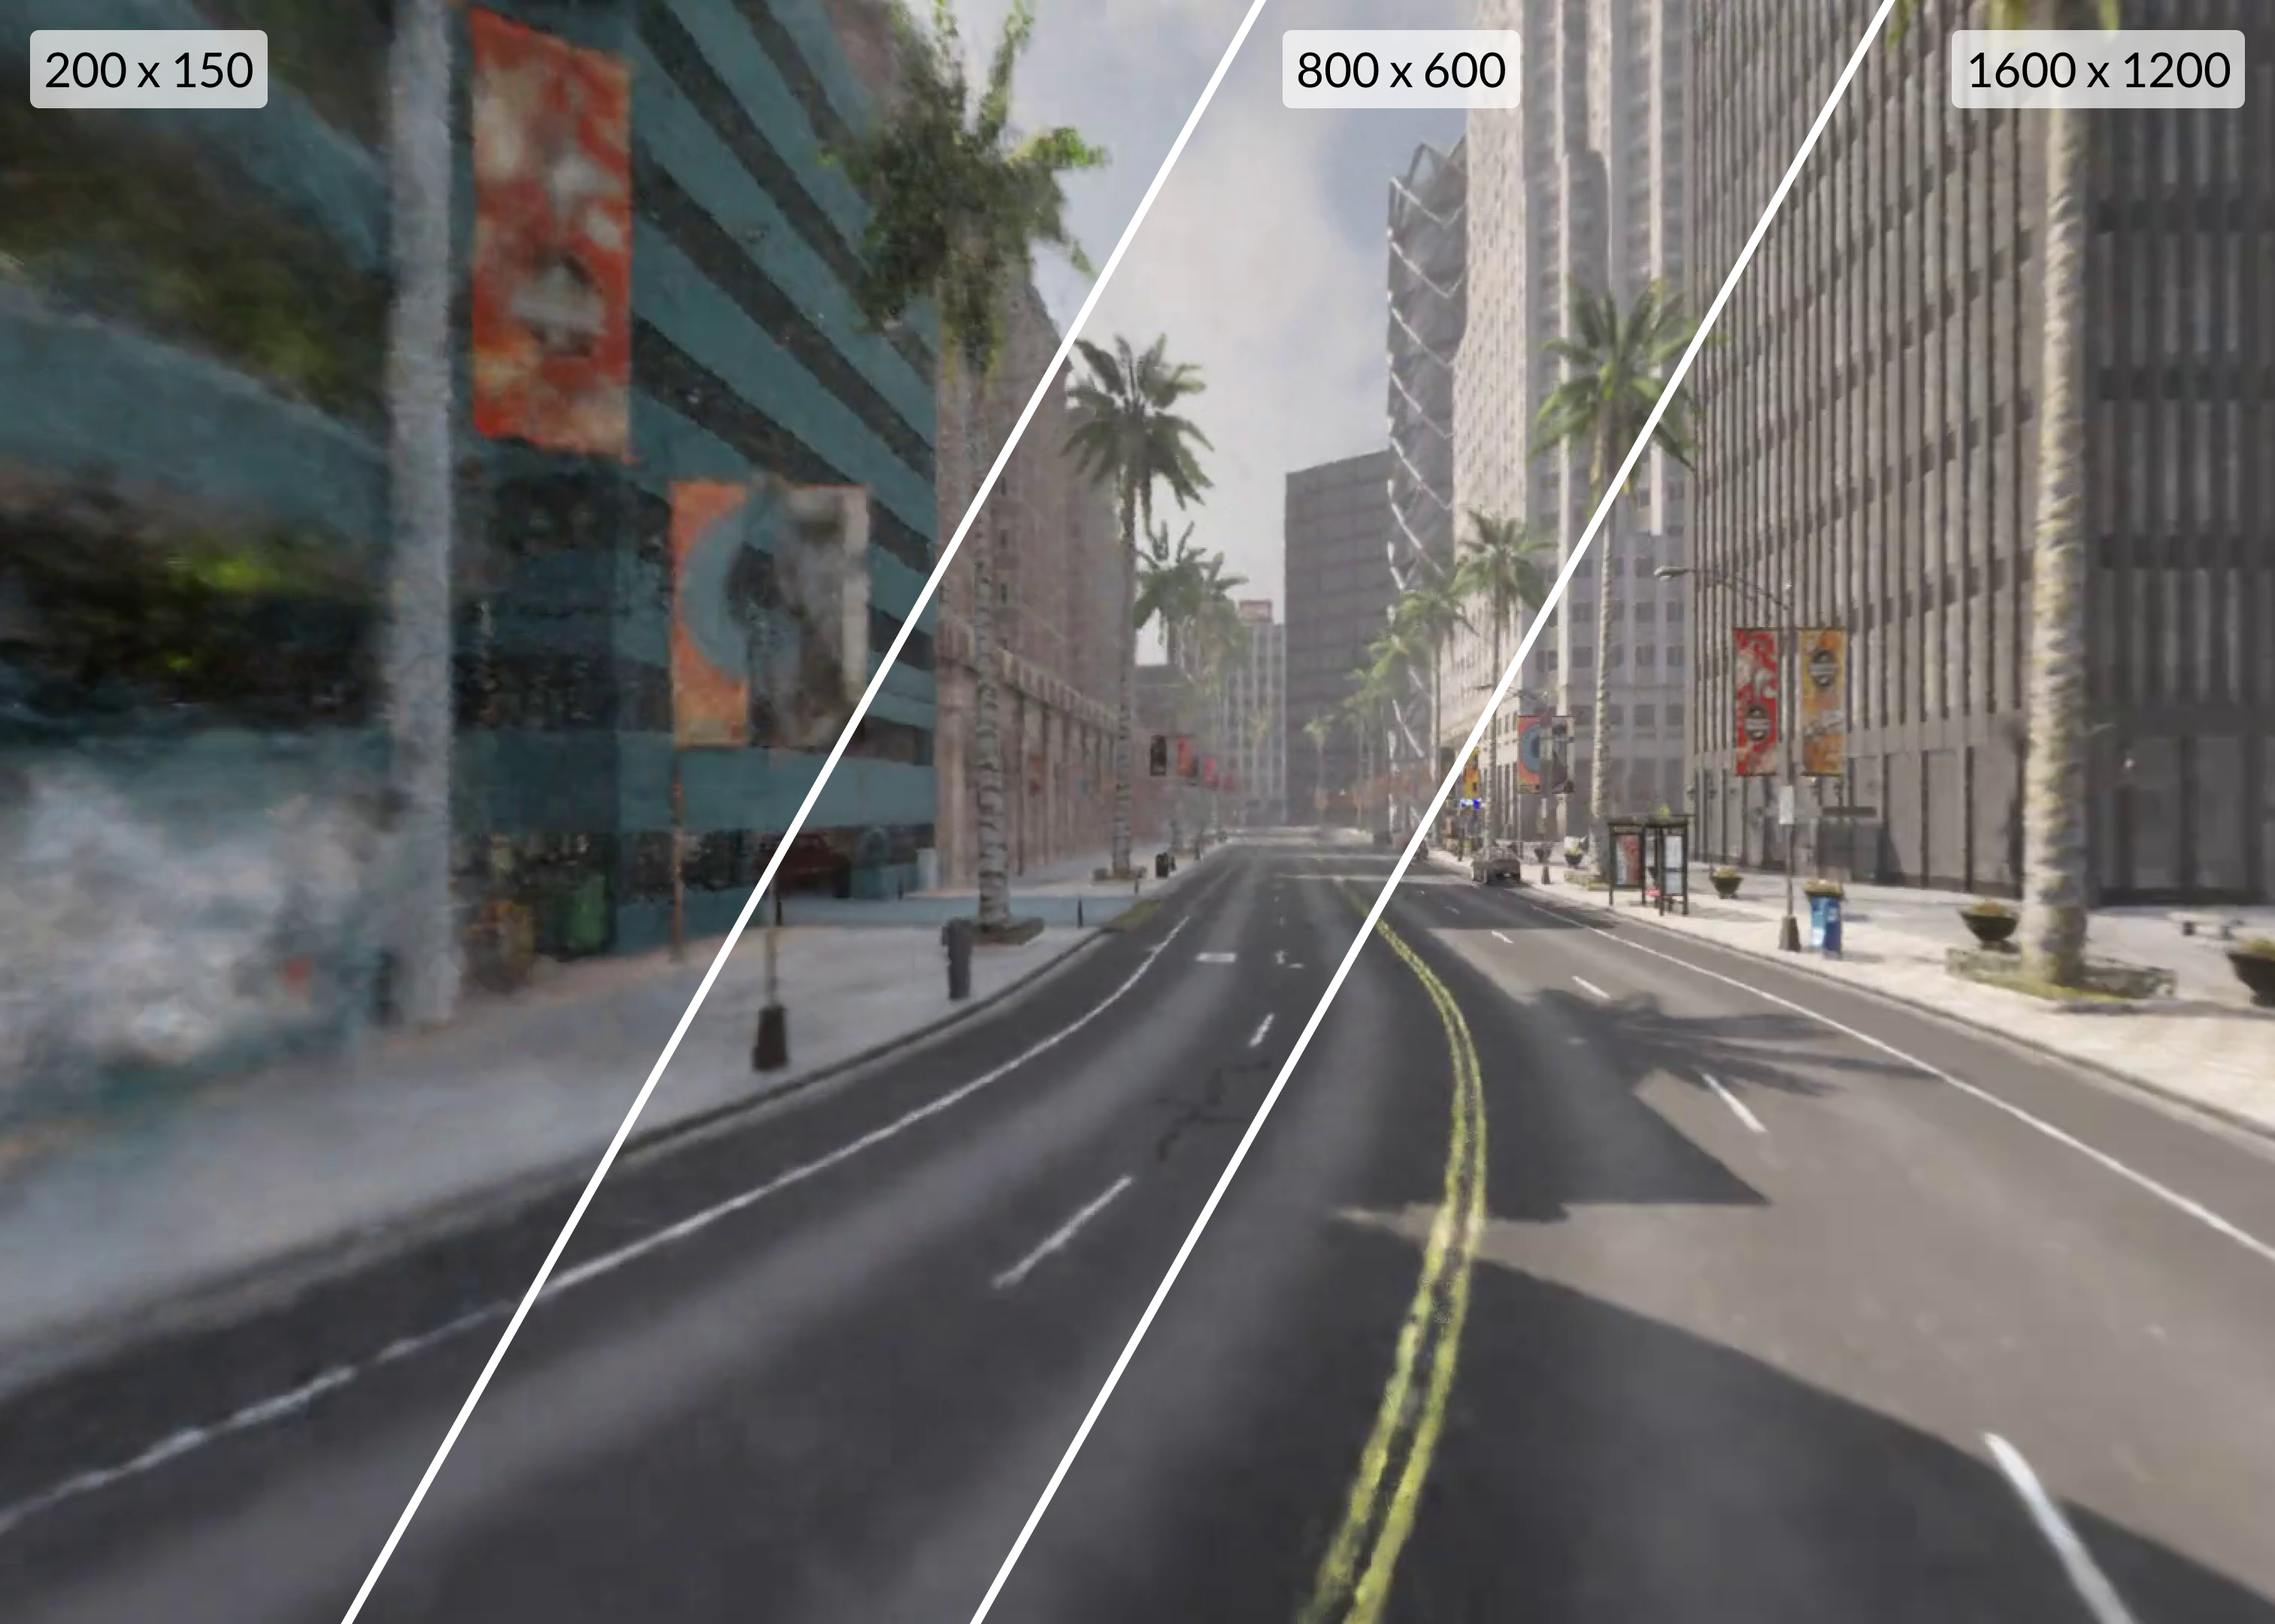
\includegraphics[width=1.0\textwidth]{figures/image-size-comparison.png}
    \caption{Comparison of frames rendered from models trained with training-data of different image resolution.}
    \label{fig:image-size-comparison}
\end{figure}

% Add to discussion
% When using lower resolution images, the LPIPS and SSIM metrics may become less sensitive because they are less affected by small differences between the synthesized and ground-truth images. This is because lower resolution images have fewer pixels, which can make the metrics less precise in measuring the perceptual similarity between the images. However, using lower resolution images can also lead to a loss of detail and fidelity in the synthesized images. When using high-resolution images, these metrics may become less effective because they are more sensitive to small differences between the synthesized and ground-truth images. In other words, the NeRF may generate high-quality images that are perceptually similar to the ground-truth images, but small differences in the pixel values or noise can cause a significant decrease in the LPIPS and SSIM scores.
% Why is there such a large difference in the LPIPS score, in contrary to the other metrics.
% - This experiment provides a clear example of how important it is to also consider the visual quality of the image synthesis and not only rely on the reported metrics.







\subsection{Experiment 1.5: Vehicle Speed} \label{sec:exp-speed}
Higher vehicle speeds result in the capture of larger portions of the scene in a shorter amount of time. However, the motion of the vehicle during capture can lead to image blurring and distortion, potentially decreasing the performance of the resulting NeRF. To investigate the impact of vehicle speed on the quality of the captured data and the resulting NeRF, we conducted a series of experiments at varying speeds.



\begin{table}[ht]
\centering
\setlength{\tabcolsep}{6pt}
\renewcommand{\arraystretch}{1.5}
\begin{tabular}{l | C{2.2} C{1.3} C{1.3}}
\hline
\textbf{Description} & \textbf{PSNR $\uparrow$} & \textbf{SSIM $\uparrow$} & \textbf{LPIPS $\downarrow$} \\
\hline
\begin{comment} New run with baseline.
\cellcolor{blue}50\% speed & \cellcolor{green} 25.326929 & \cellcolor{green} 0.817911 & \cellcolor{red} 0.216335 \\
100\% speed & 25.158533 & 0.815676 & \cellcolor{green} 0.196946 \\
150\% speed & \cellcolor{red} 24.612526 & \cellcolor{red} 0.800840 & 0.205222 \\
200\% speed & 25.007772 & 0.801815 & 0.197255 \\
\end{comment}
\cellcolor{blue}50\% speed & \cellcolor{green} 24.061440 & \cellcolor{green} 0.775393 & \cellcolor{green} 0.181360 \\
100\% speed & 23.502066 & 0.755476 & 0.184455 \\
150\% speed & 23.411259 & 0.742473 & 0.189968 \\
200\% speed & \cellcolor{red} 22.717318 & \cellcolor{red} 0.713858 & \cellcolor{red} 0.200099 \\
\end{tabular}
\caption[Results for experiment 1.5: Vehicle speed]{Comparison of different vehicle speeds' impact on the NeRF's performance. CARLA convention conveys speed as a percentage of the default speed of 30 km\/h.}
\label{tab:exp_speed-2}
\end{table}

\begin{comment}
\vspace{0.5cm}

\setlength{\tabcolsep}{12pt}
\renewcommand{\arraystretch}{1.2}
\begin{tabular}{l l}
\multicolumn{2}{c}{\textbf{Experiment setup - constant variables}} \\
\hline
Parameter & Value \\
\hline
\cellcolor{blue}Camera setup &\cellcolor{blue}Two cameras, $[-10^{\circ}, 10^{\circ}]$ yaw  \\
\cellcolor{blue}Distance &\cellcolor{blue}4 turns \\
\cellcolor{blue}Ticks per image &\cellcolor{blue}Capture data every 2$^{\text{nd}}$ tick \\
\cellcolor{blue}Image resolution &\cellcolor{blue}Image resolution of $400 \times 300$ \\
\hline
\end{tabular}
\caption[Constant parameters for experiment 1.5.]{Overview of the values of the parameters that remained constant across the experiments' runs.}
\label{tab:exp-speed-stable-variables}
\end{comment}

The results of the experiments, presented in \autoref{tab:exp_speed-2}, indicate that the speed of the vehicle significantly impacts the quality of the data captured by the mounted cameras. Specifically, we observe that the NeRF trained on the data captured at 50\% speed achieves the highest scores on all three metrics (\acrshort{psnr}, \acrshort{ssim}, and \acrshort{lpips}), while the NeRF trained on the data captured at 200\% speed achieves the lowest scores on all three metrics. These findings suggest that slower vehicle speeds can lead to higher-quality data capture, while faster vehicle speeds can lead to lower-quality data capture. As a result, the configuration of 50\% reduced vehicle speed was selected for further experiments.



% For the discussion-section
% The reason for this can be attributed to the motion blur and temporal artifacts that can occur when the vehicle is moving too fast. At higher speeds, the motion of the vehicle can cause blurring and distortion in the captured images, which can reduce the quality of the data and make it more difficult for the NeRF to learn the underlying 3D scene structure and appearance. In contrast, slower vehicle speeds can reduce the amount of motion blur and temporal artifacts, resulting in clearer and more detailed images. Another side effect of driving slower is that it leads to increased amount of images captured. At 50\% speed, the dataset consists of 351 images, in contrast to the 131 images captured at 200\% speed.













\subsection{Experiment 1.6: Assessing the Combined Baseline} \label{sec:exp-combined-baseline}
The configurations selected for the baseline used in further experiments are a combination of the configurations that produced the best results across the previous experiments. The baseline’s distance is the only setting that deviates from the configurations that produced the best results in previous experiments, and it will remain constant with a full lap around the block. As a result, the baseline's configurations consist of two forward-facing RGB-cameras, counterrotated with $-10^\circ$- and $10^\circ$ yaw, capturing data every second tick, along a city-block that spans $\sim450$ meters in distance, with an image size of $400 \times 300$, and a vehicle speed that's 50\% slower than the default of 30 km/h. 

The baseline's high scores across all three metrics, \acrshort{psnr}, \acrshort{ssim}, and \acrshort{lpips}, as presented in \autoref{tab:exp_combined_baseline_2-0}, demonstrate that this configuration yields high-quality data capture. As a result, the combined baseline can serve as a useful starting point for future research and applications.


\begin{table}[ht]
\centering
\setlength{\tabcolsep}{6pt}
\renewcommand{\arraystretch}{1.5}
\begin{tabular}{l | C{2.2} C{1.3} C{1.3}}
\hline
\textbf{Description} & \textbf{PSNR $\uparrow$} & \textbf{SSIM $\uparrow$} & \textbf{LPIPS $\downarrow$} \\
\hline
Combined baseline & 24.197817 & 0.766733 & 0.168807 \\
\hline
\end{tabular}
\caption[Results for experiment 1.6: Combined baseline]{The baseline metrics for a Nerfacto model trained on synthetic data captured from CARLA.}
\label{tab:exp_combined_baseline_2-0}

\vspace{0.5cm}

\setlength{\tabcolsep}{12pt}
\renewcommand{\arraystretch}{1.5}
\begin{tabular}{l | l}
\hline
\textbf{Parameter} & \textbf{Value} \\
\hline
\cellcolor{blue}Camera setup &\cellcolor{blue}Two cameras, $[-10^{\circ}, 10^{\circ}]$ yaw  \\
\cellcolor{blue}Distance &\cellcolor{blue}4 turns \\
\cellcolor{blue}Ticks per image &\cellcolor{blue}Capture data every 2$^{\text{nd}}$ tick \\
\cellcolor{blue}Image resolution &\cellcolor{blue}Image resolution of $400 \times 300$ \\
\cellcolor{blue}Speed &\cellcolor{blue}50\% speed \\
\hline
\end{tabular}
\caption[Configurations for the baseline data capture]{Overview of the configurations that were selected to be part of the baseline data capture configuration, based on the results from the previous experiments.}
\label{tab:exp-combined-baseline-stable-variables}
\end{table}















%\section{Experiment 2: Camera Poses With Simulated Inaccuracies}
\section{Experiment 2: Simulated Noise Conditions}
% The NAPLab vehicle is equipped with two Swift Navigation Duro Ruggedized Receivers, which offer superior positioning accuracy compared to regular GPS/GNSS systems. According to the manufacturer’s documentation, each Duro module has a horizontal position accuracy of 0.75 meters (CEP 50 in SBAS mode) without RTK, and can achieve centimeter-level accuracy with RTK enabled. This high level of accuracy enables the capture of rough camera poses alongside image capturing.

During the capture of images and corresponding camera poses from a vehicle in a real-world scenario, the accuracy of camera poses is often impaired, primarily due to imperfections in \acrshort{gps}/\acrshort{gnss}-readings. To investigate the impact of noisy camera poses and the effectiveness of camera pose optimization, an experiment was conducted in which Gaussian noise was introduced to the camera poses obtained from the CARLA pipeline. The addition of Gaussian noise to the camera poses simulates the effects of imperfect camera poses in real-world data capture. The magnitude of the added noise is determined by the standard deviation of the Gaussian distribution, which increases progressively throughout the experiments. The results for the runs with and without camera optimization are presented in \autoref{tab:exp-gaussian-noise} and \autoref{fig:noise-combined-comparison}, with a full table of additional increments in \autoref{app:noise}.

% I've tried combining both the baseline and shorter segments into single table.
\begin{table}[ht]
\centering
\setlength{\tabcolsep}{6pt}
\renewcommand{\arraystretch}{1.5}
\begin{tabular}{l | C{2.2} C{1.3} C{1.3} | C{2.2} C{1.3} C{1.3}}
\hline
\textbf{Description} & \textbf{PSNR $\uparrow$} & \textbf{SSIM $\uparrow$} & \textbf{LPIPS $\downarrow$} & \textbf{PSNR $\uparrow$} & \textbf{SSIM $\uparrow$} & \textbf{LPIPS $\downarrow$} \\
\hline
& \multicolumn{6}{c}{\textbf{Baseline segment}} \\
\hline
& \multicolumn{3}{c|}{\textbf{With camera optimizer}} & \multicolumn{3}{c}{\textbf{Without camera optimizer}} \\
\hline
$\mathcal{N}(0, 0.0)$   & 23.412970 & 0.713507 & 0.320640 &\cellcolor{green} 24.702831 &\cellcolor{green} 0.792646 &\cellcolor{green} 0.179289 \\
$\mathcal{N}(0, 0.1^2)$ & 22.513981 & 0.674136 & 0.321364 & 22.463675 & 0.677371 & 0.280633 \\
$\mathcal{N}(0, 0.5^2)$ & 19.075649 & 0.501499 & 0.371572 & 19.366894 & 0.499264 & 0.474444 \\
$\mathcal{N}(0, 1.0^2)$ & 17.670620 & 0.433909 & 0.432940 & 18.207266 & 0.444120 & 0.560452 \\
$\mathcal{N}(0, 3.0^2)$ & 16.662760 & 0.408036 & 0.637326 &\cellcolor{red} 16.322678 &\cellcolor{red} 0.385614 &\cellcolor{red} 0.647966 \\
\hline
& \multicolumn{6}{c}{\textbf{Shorter segment}} \\
\hline
& \multicolumn{3}{c|}{\textbf{With camera optimizer}} & \multicolumn{3}{c}{\textbf{Without camera optimizer}} \\
\hline
$\mathcal{N}(0, 0.0)$   & 24.831890 & 0.824606 & 0.102266 &\cellcolor{green} 25.677803 &\cellcolor{green} 0.861634 &\cellcolor{green} 0.076989 \\ 
$\mathcal{N}(0, 0.1^2)$ & 23.028709 & 0.752731 & 0.114806 & 23.318026 & 0.755237 & 0.146877 \\ 
$\mathcal{N}(0, 0.5^2)$ & 19.059755 & 0.482721 & 0.197262 & 20.071671 & 0.513037 & 0.299472 \\ 
$\mathcal{N}(0, 1.0^2)$ & 18.085838 & 0.406564 & 0.338364 & 18.290358 & 0.417969 & 0.404933 \\ 
$\mathcal{N}(0, 3.0^2)$ & 15.709220 &\cellcolor{red} 0.344876 & 0.612587 &\cellcolor{red} 15.077240 & 0.362973 &\cellcolor{red} 0.698665 \\ 
\hline
\end{tabular}
\caption[Results for experiment 2: Adding noise]{Results for Gaussian Noise experiment on both the baseline and shorter segments. The shorter segment is 10\% the size of the baseline segment, approximately 50m in length.}
\label{tab:exp-gaussian-noise}
\end{table}

%\begin{figure}[!h]
    \centering
    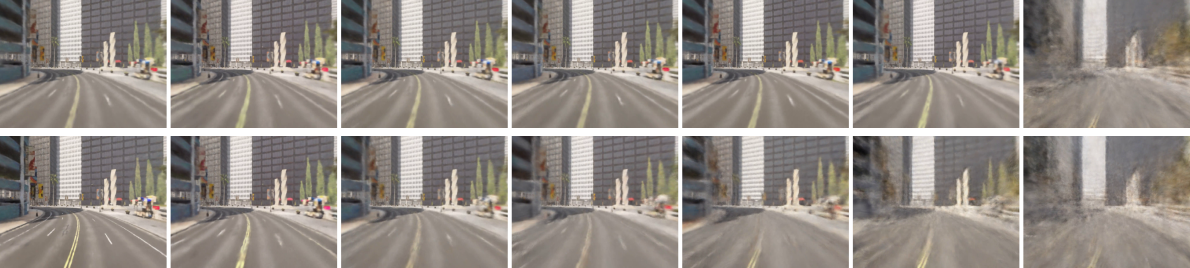
\includegraphics[width=1.0\textwidth]{figures/noise-baseline-segments.png}
    \caption{Comparison of the effect of noise on the camera poses. The top row utilizes camera optimization, while the second row doesn't.}
    \label{fig:noise-baseline-segments}
\end{figure}
%\begin{figure}[!h]
    \centering
    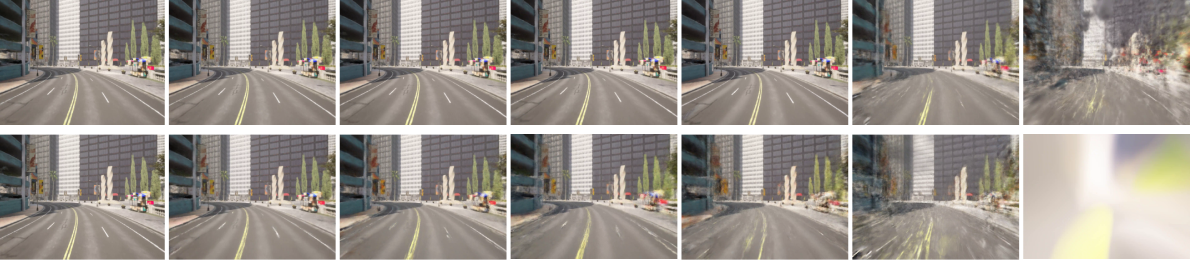
\includegraphics[width=1.0\textwidth]{figures/noise-short-segments.png}
    \caption{Comparison of the effect of noise on the camera poses. The top row utilizes camera optimization, while the second row does not.}
    \label{fig:noise-short-segments}
\end{figure}
\begin{figure}[!h]
    \centering
    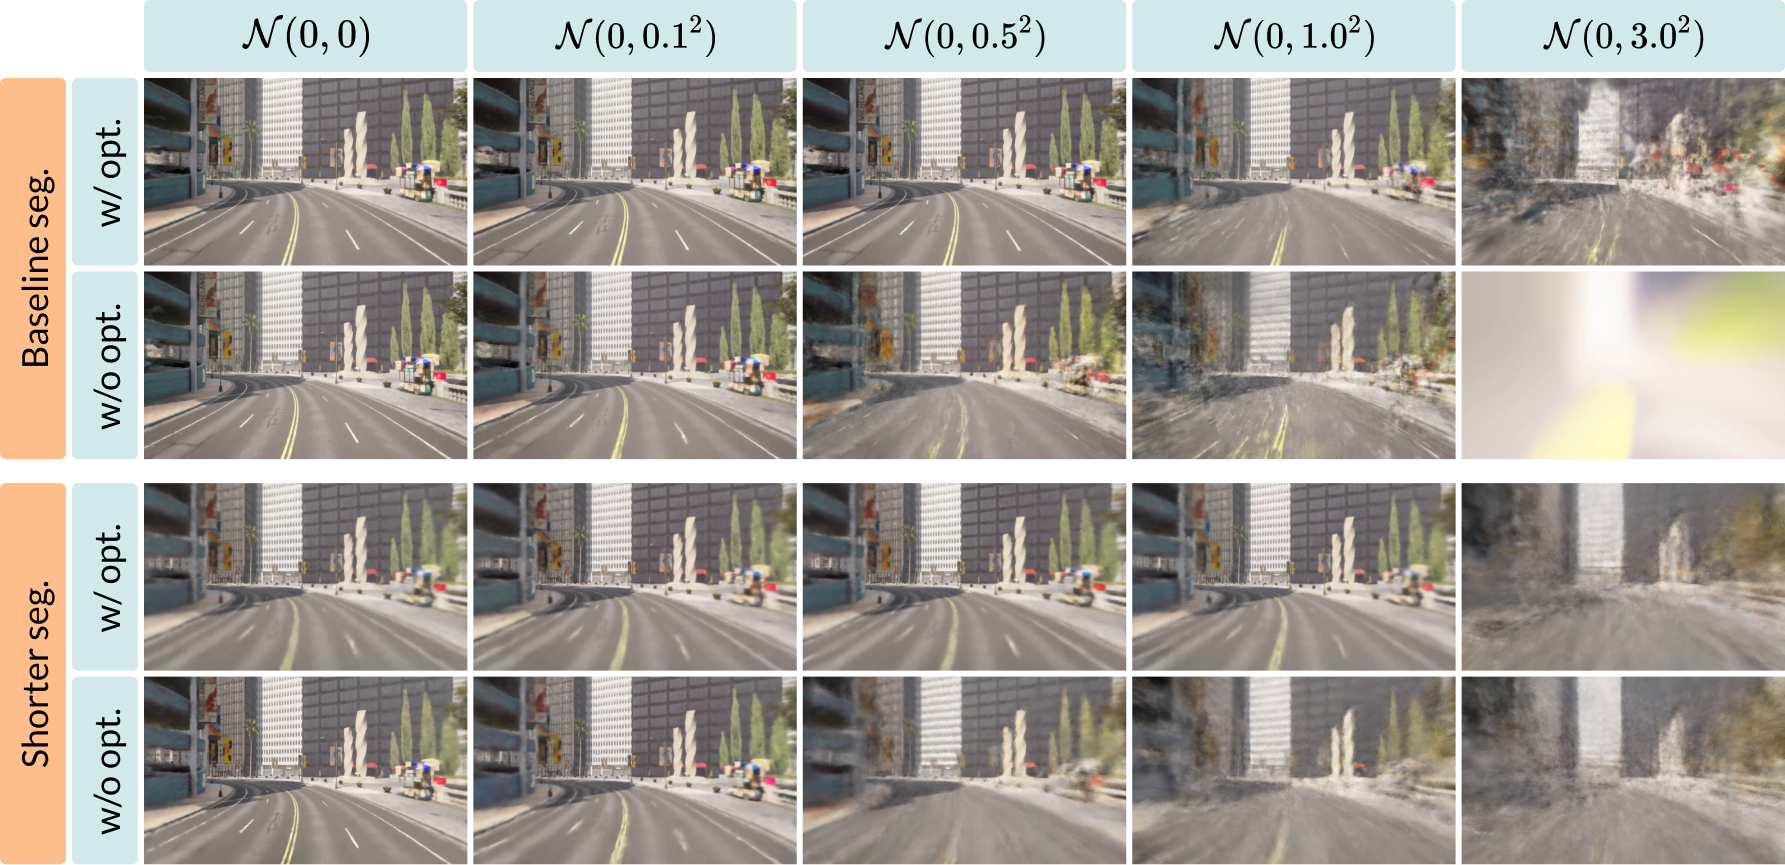
\includegraphics[width=1.0\textwidth]{figures/noise-combined-comparison.png}
    \caption[Qualitative assessment of NeRF trained on noisy dataset.]{Comparison of the effect of simulated noise conditions for the trained NeRF.}
    \label{fig:noise-combined-comparison}
\end{figure}

The NeRF's quality degrade across all metrics as the noise increases. While the difference in quantitative results between the runs with and without camera pose optimization may appear small, the qualitative comparison depicted in \autoref{fig:noise-combined-comparison} provides clear evidence of the optimization's efficacy. In addition, it seems to have a more substantial impact on shorter segments, than larger ones.

\begin{comment}
Information about GNSS-error
https://junipersys.com/support/article/6614#:~:text=Just%20as%20a%20general%20observation,to%202%20m%20vertical%20accuracy.
\end{comment}

% Discuss in discussion
% - Hypothesis: The camera optimization works better on short segments, which entails that Block-NeRF will have an even greater benefit when the scene is large.
% - Interestingly the run with no added noise and no camera optimizer performs better on all metrics than the same run with camera optimizer. I believe this is because the camera optimizer might "blur" the already perfect camera poses.
% - From the quantitative assessment, it doesn't seem like the camera optimizer does much for the longer segments.


\subsection{Experiment 2.1: COLMAP versus Camera Pose Optimization}

The camera optimization in the previous experiment shows promising results. In order to further investigate the effect of direct camera optimization on vehicle-captured data, a comparison to COLMAP's result on the same dataset is conducted. \autoref{tab:colmap-vs-poses} presents the results from the NeRF trained on the same images as in the experiment above, but with camera poses approximated with the SfM tool COLMAP.

\begin{table}[ht]
\centering
\setlength{\tabcolsep}{6pt}
\renewcommand{\arraystretch}{1.5}
\begin{tabular}{l | C{2.2} C{1.3} C{1.3} c}
\hline
\textbf{Description} & \textbf{PSNR $\uparrow$} & \textbf{SSIM $\uparrow$} & \textbf{LPIPS $\downarrow$} & \textbf{Time processing} \\
\hline
COLMAP - Baseline segment   & 24.18618  & 0.758549  & 0.159935  & 01:12:15 \\
COLMAP - Shorter segment    & 25.227386 & 0.8273112 & 0.0932542 & 00:02:00 \\
\hline
\end{tabular}
\caption[Results for experiment 2.1: COLMAP]{Results for approximating camera poses with COLMAP for the baseline and short segment.}
\label{tab:colmap-vs-poses}
\end{table}

\begin{comment}
\begin{table}[ht]
\centering
\setlength{\tabcolsep}{6pt}
\renewcommand{\arraystretch}{1.5}
\begin{tabular}{l | C{2.2} C{1.3} C{1.3} c}
\hline
\textbf{Description} & \textbf{PSNR $\uparrow$} & \textbf{SSIM $\uparrow$} & \textbf{LPIPS $\downarrow$} & \textbf{Time processing} \\
\hline
\multicolumn{5}{c}{Baseline segment} \\
\hline
CARLA w/o camera optimization & \cellcolor{green} 24.702831268310547 & \cellcolor{green} 0.7926456332206726 & \cellcolor{red} 0.17928948998451233  & 00:00:00 \\
CARLA w/ camera optimization & 24.197817 & 0.766733 & 0.168807 & 00:00:00 \\% exp\_combined\_baseline\_2-0
COLMAP & \cellcolor{red} 24.18618 & \cellcolor{red} 0.758549 & \cellcolor{green} 0.159935 & 01:12:15 \\% data-images-exp\_combined\_baseline\_2\_colmap
\hline
\multicolumn{5}{c}{Shorter segment - 10\% of baseline} \\
\hline
CARLA w/o camera optimization &\cellcolor{green} 25.677803 & \cellcolor{green} 0.861634 & \cellcolor{green} 0.076989  & 00:00:00 \\
CARLA w/ camera optimization &\cellcolor{red} 24.831890 &\cellcolor{red} 0.824606 &\cellcolor{red} 0.102266 & 00:00:00 \\
COLMAP & 25.227386 & 0.8273112 & 0.0932542 & 00:02:00 \\
\hline
\end{tabular}
\caption{Results for experiments}
\label{tab:colmap-vs-poses}
\end{table}
\end{comment}


First, looking back at the results in \autoref{tab:exp-gaussian-noise}, we observe that small amounts of noise severely degrade the quality of the NeRF even when the camera poses are optimized throughout the NeRF's training. Comparing those results with COLMAP's results on the same datasets as depicted in \autoref{tab:colmap-vs-poses}, it becomes apparent that although direct pose optimization offers the benefit of avoiding pre-processing, the NeRF trained with camera poses approximated by COLMAP consistently delivers superior performance across all metrics when the camera poses are noisy, regardless of segment size. The results thus suggest that employing COLMAP for initial pose approximation could significantly improve model performance when the initial camera poses are inaccurate, despite the longer processing time required.


\begin{comment}
This subsection presents an experiment designed to assess the relative merits of two distinct strategies for refining initial camera poses. Specifically, we compare the direct optimization of rough camera poses within the model training pipeline against the pre-processing of such poses with the help of COLMAP. The main question under investigation here is whether the benefits of optimizing the rough camera poses directly can outweigh those of employing a sophisticated SfM tool like COLMAP, despite the potential for a more substantial time investment.

might offer the benefit of faster processing time, COLMAP consistently delivers superior performance across all metrics, regardless of segment size.
COLMAP doesn't optimize initial poses, but instead approximates camera poses from a set of input images. 
Comparing those results with \autoref{tab:colmap-vs-poses}, we observe that the runs with poses approximated by COLMAP deliver superior performance
Comparing the results in \autoref{tab:colmap-vs-poses} and \autoref{tab:exp-gaussian-noise} it becomes apparent that although direct pose optimization might offer the benefit of faster processing time, COLMAP consistently delivers superior performance across all metrics, regardless of segment size. The results thus suggest that employing COLMAP for initial pose refinement could significantly improve model performance when the initial camera poses are inaccurate, despite the longer processing time required.
\end{comment}











\newpage

\section{Experiment 3: Comparing Different Models}
Nerfstudio has implemented multiple well-known NeRF-models including Instant-ngp \cite{mullerInstantNeuralGraphics2022} and Mip-NeRF \cite{barronMipNeRFMultiscaleRepresentation2021}. In this experiment, we investigate the model's impact on the output. The comparison of the different models is presented in \autoref{tab:different-models} and \autoref{fig:different-models}.

\begin{table}[ht]
\centering
\setlength{\tabcolsep}{6pt}
\renewcommand{\arraystretch}{1.5}
\begin{tabular}{l | C{2.2} C{1.3} C{1.3} | r}
\hline
\textbf{Description} & \textbf{PSNR $\uparrow$} & \textbf{SSIM $\uparrow$} & \textbf{LPIPS $\downarrow$} & Iterations \\
\hline
Nerfacto        & 24.197817                     &\cellcolor{green} 0.766733     &\cellcolor{green} 0.168807 & 15'000 \\
Instant-ngp     &\cellcolor{green} 24.253278   & 0.7564714                     & 0.231680 & 15'000 \\
Nerfacto-big    & 23.5648784     & 0.74144792     & 0.2829464 & 100'000 \\
Mip-NeRF        &\cellcolor{red} 9.487646 &\cellcolor{red} 0.165382 &\cellcolor{red} 0.775073 & 300'000 \\
\hline
\end{tabular}
\caption[Results for experiment 3: Different models]{The result of training different models implemented in the Nerfstudio framework on the combined baseline dataset.}
\label{tab:different-models}
\end{table}

\begin{figure}[ht]
    \centering
    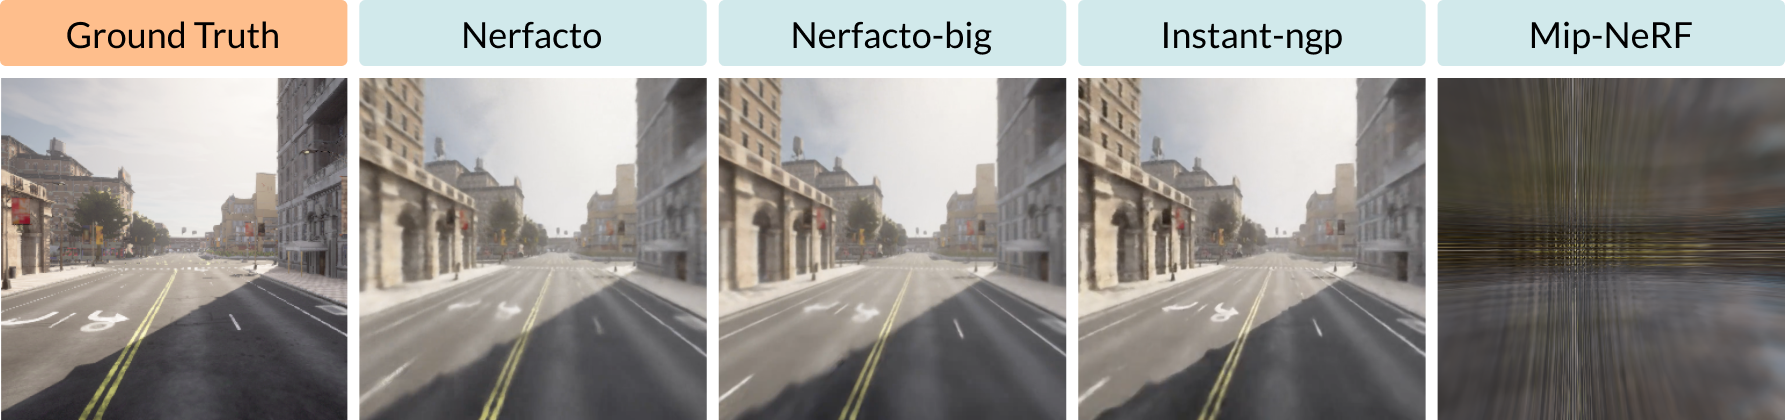
\includegraphics[width=1.0\textwidth]{figures/different-models.png}
    \caption{Qualitative comparison of different NeRF-models.}
    \label{fig:different-models}
\end{figure}

The quantitative results indicate that there are no significant differences between the fast methods, Nerfacto, Nerfacto-big, or Instant-ngp. However, both the quantitative and qualitative results reveal that the Mip-NeRF model is unable to learn the unbounded scene, resulting in the worst scores across all metrics.









\section{Experiment 4: Large-Scale NeRF}

The naive Block-NeRF implementation allows for the captured scene to be split into an arbitrary number of segments. In this experiment, we'd like to explore the impact of splitting the scene on the overall quality of the generated results. In particular, we compare the performance of Block-NeRF to that of a single NeRF trained on the entire scene. \autoref{tab:exp_combined_baseline_block_nerf} shows the result of splitting the baseline-scene into 4 segments, while \autoref{tab:exp_block_nerf_long_path_2-block_10} shows the result of splitting a larger scene, a trajectory of approximately 1200 meters, into 12 segments. The qualitative results of the 12-segment run can be seen in \autoref{fig:block-nerf-comparison}.

%By splitting the scene into smaller segments, the combined scene generates better results than when the entire scene is trained within a single NeRF. The average PSNR is 24.4746 - which is 0.2768 better than the entire scene in one. Block-NeRF's high quality will sustain large scenes, where a single NeRF will start deteriorating as the scene size increases.

\begin{table}[ht]
\centering
\setlength{\tabcolsep}{6pt}
\renewcommand{\arraystretch}{1.5}
\begin{tabular}{l | C{2.2} C{1.3} C{1.3}}
\hline
\textbf{Description} & \textbf{PSNR $\uparrow$} & \textbf{SSIM $\uparrow$} & \textbf{LPIPS $\downarrow$} \\
\hline
Average across 4 Block-NeRFs &\cellcolor{green} 24.4746415 &\cellcolor{green} 0.78977125 &\cellcolor{red} 0.1841015 \\
Single NeRF &\cellcolor{red} 24.197817 &\cellcolor{red} 0.766733 &\cellcolor{green} 0.168807 \\
\hline
%Average difference from one NeRF &\cellcolor{green} 0.2768 &\cellcolor{green} 0.02277125 &  \cellcolor{red} -0.015 % Unsure if I'll include this
\end{tabular}
\caption[Results for experiment 4: Block-NeRF on 4-segment dataset]{The average metrics across the four segments compared to the combined baseline on the same scene. The full overview of each segment's metrics can be viewed in the appendix in \autoref{tab:block-nerf-four-segments-full}.}
\label{tab:exp_combined_baseline_block_nerf}
\end{table}


\begin{table}[ht]
\centering
\setlength{\tabcolsep}{6pt}
\renewcommand{\arraystretch}{1.5}
\begin{tabular}{l | C{2.2} C{1.3} C{1.3}}
\hline
\textbf{Description} & \textbf{PSNR $\uparrow$} & \textbf{SSIM $\uparrow$} & \textbf{LPIPS $\downarrow$} \\
\hline
Average across 12 Block-NeRFs & \cellcolor{green} 24.774259 & \cellcolor{green} 0.801090 & \cellcolor{green} 0.159331 \\
Single NeRF & \cellcolor{red} 22.515461 & \cellcolor{red} 0.654036 & \cellcolor{red} 0.424356 \\
\hline
\end{tabular}
\caption[Results for experiment 4: Block-NeRF on 12-segment dataset]{The average metrics across the twelve segments compared to the metrics for a single NeRF trained on the same scene. The full overview of each segment's metrics can be viewed in the appendix in \autoref{tab:block-nerf-twelve-segments-full}.}
\label{tab:exp_block_nerf_long_path_2-block_10}
\end{table}
\begin{figure}[!h]
    \centering
    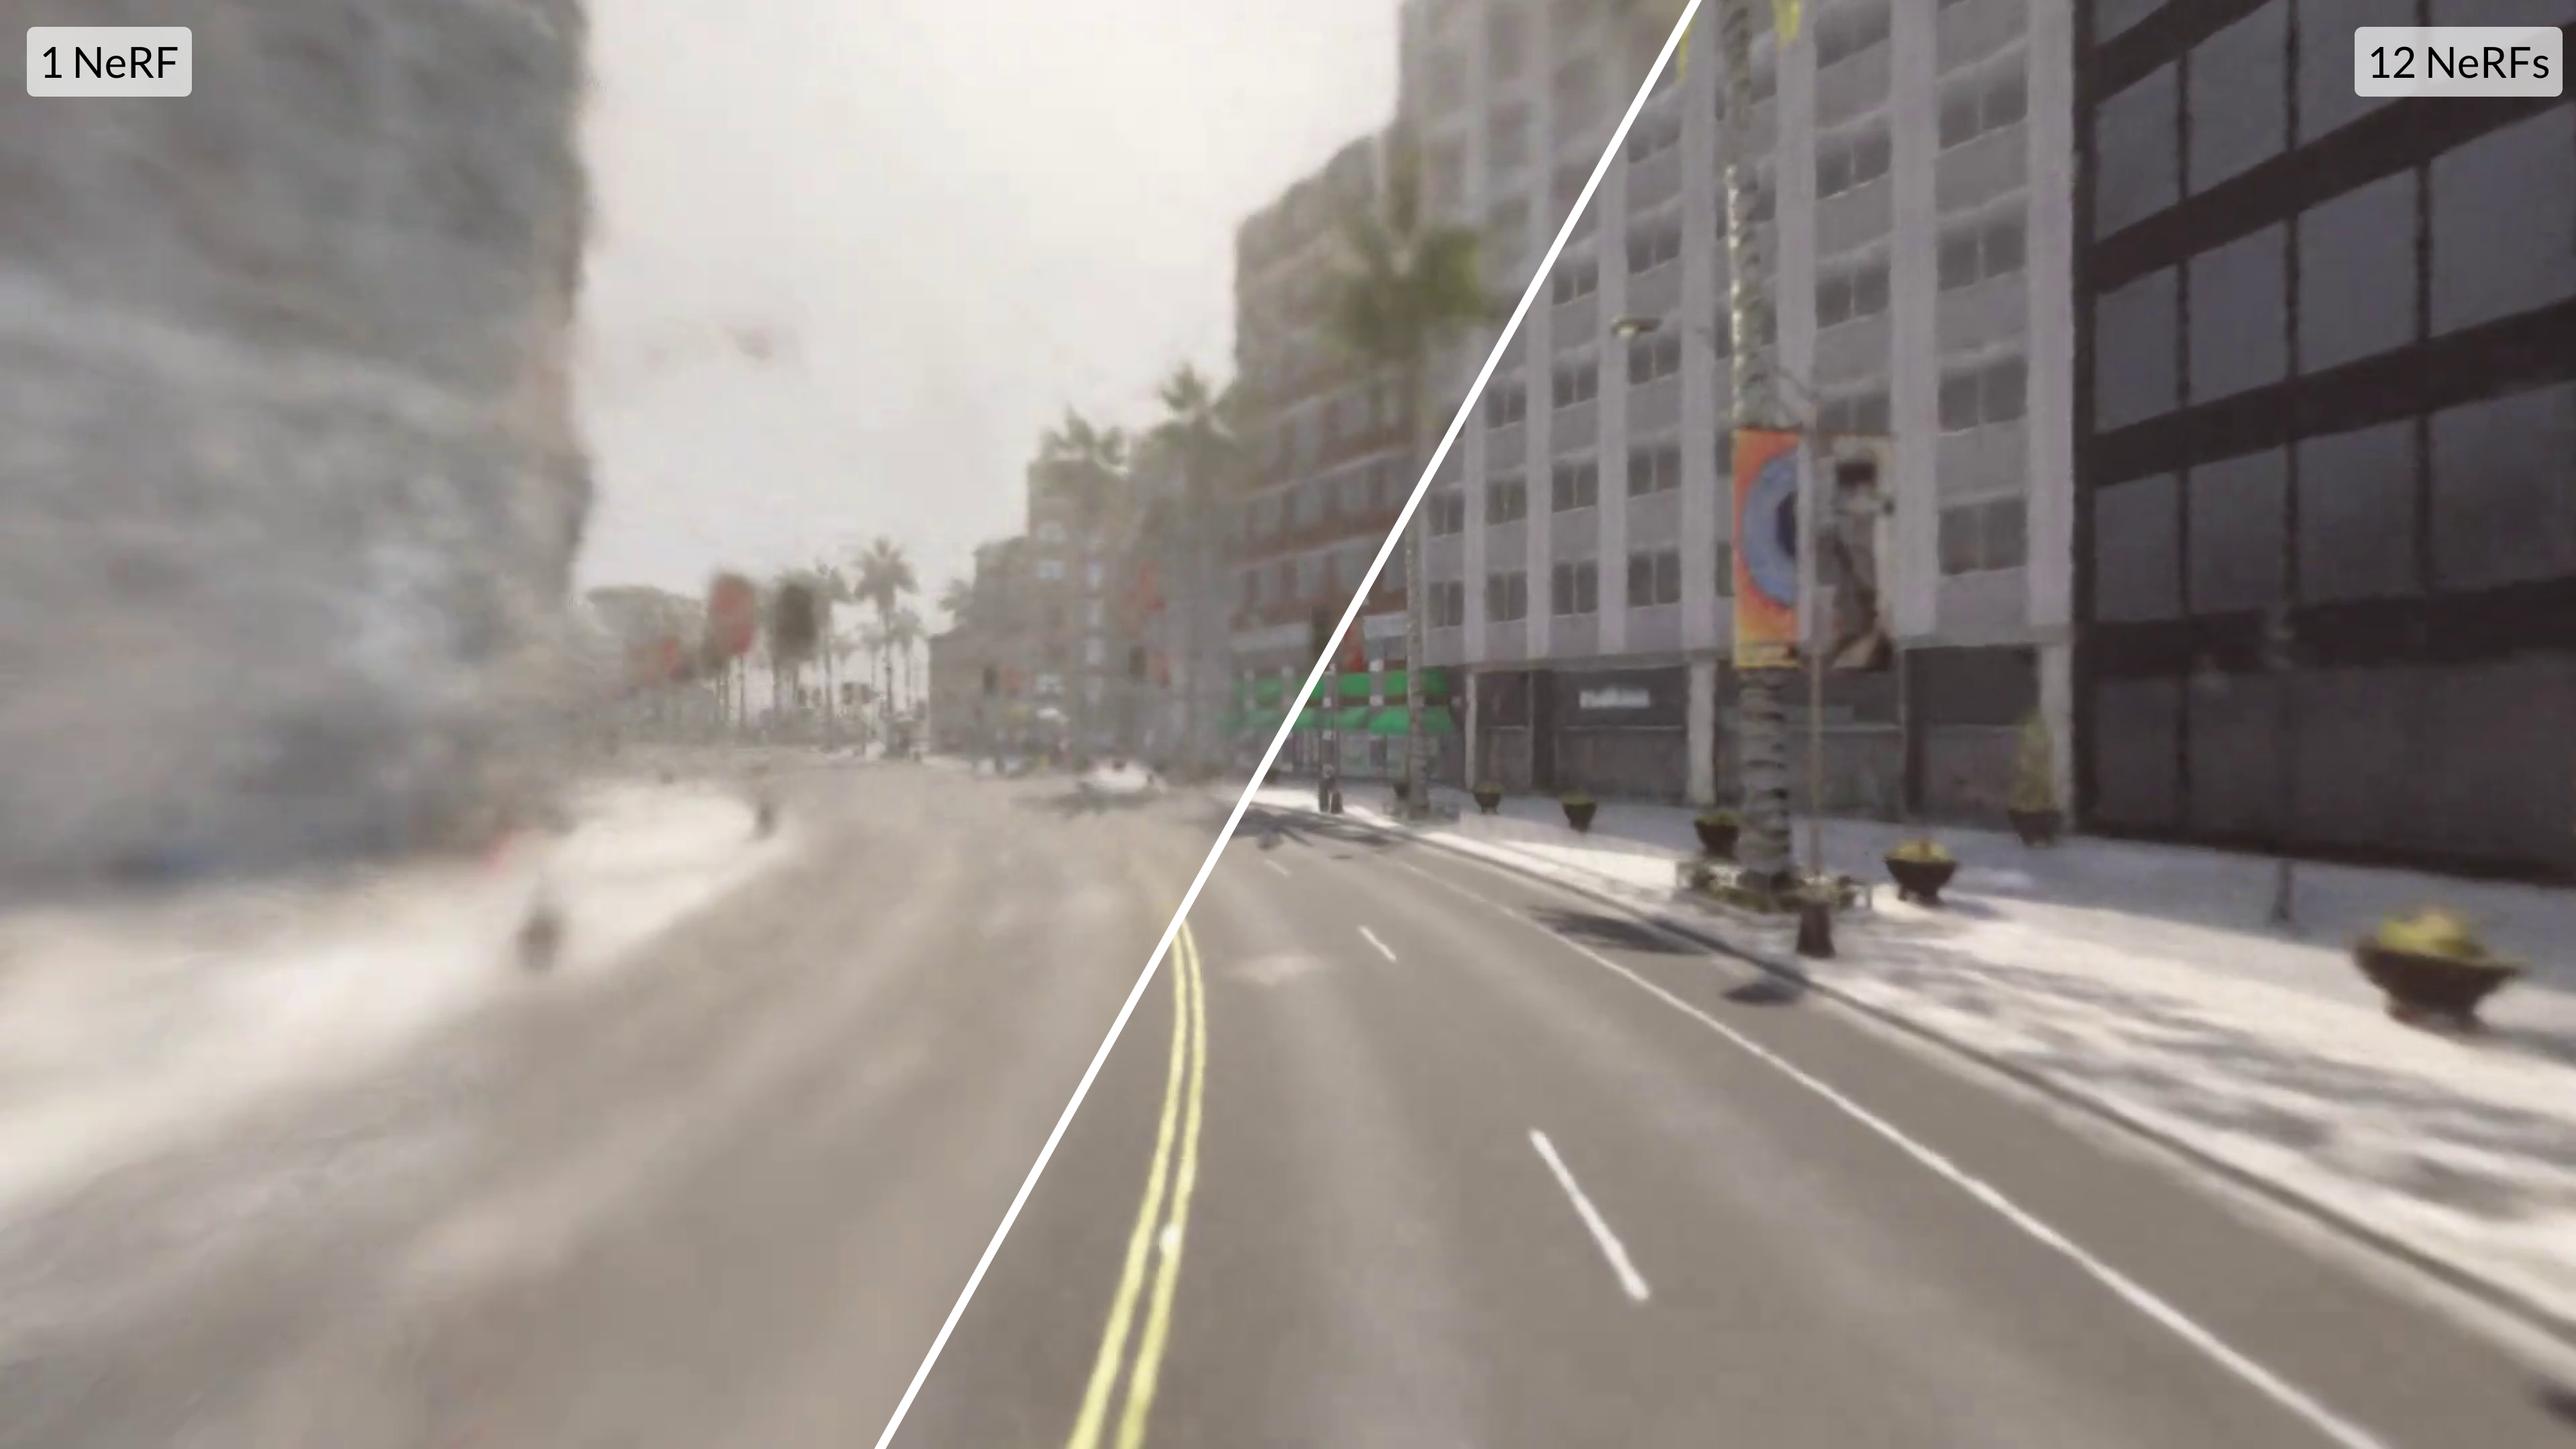
\includegraphics[width=1.0\textwidth]{figures/block-nerf-comparison.png}
    \caption{Comparison of two renders from models who have been trained on the same data. Left) One NeRF trained on all data, Right) 12 NeRFs trained on equally spaced segments.}
    \label{fig:block-nerf-comparison}
\end{figure}

The experimental findings indicate that the naive Block-NeRF implementation enables high-quality image synthesis across large scenes, while a single NeRF trained on the same large scene experiences a decline in performance, resulting in poor image synthesis quality. These results suggest that Block-NeRF represents a promising approach for generating high-quality results for large-scale scenes.

\subsection{Experiment 4.1: Removing Artifacts}
Despite the significantly lower quality of the single NeRF implementation compared to the Block-NeRF implementation, the resulting render exhibits clear coherence without sudden changes in detail or the abrupt appearance of artifacts. In contrast, the naive Block-NeRF implementation suffers from this issue, as illustrated in \autoref{fig:block-nerf-frame-comparison}.

\begin{figure}[!h]
    \centering
    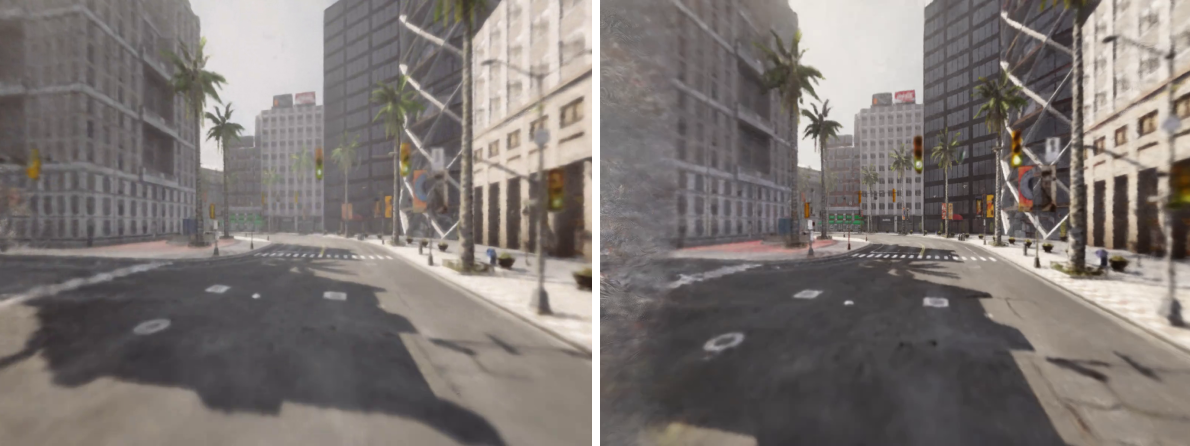
\includegraphics[width=1.0\textwidth]{figures/block-nerf-frame-comparison.png}
    \caption{Comparison of two consecutive frames of a single render on a 12 block NeRF. The first frame (left) is the last frame rendered by block number 1. The second frame (right) is the first frame rendered by block number 2. The details of the scenery in the second frame is clearly better than the first, which is expected as block number 2 have been trained on close-up images of the scene. This difference could be mitigated by looking into image merging techniques such as inverse distance weighing.}
    \label{fig:block-nerf-frame-comparison}
\end{figure}

This issue could possibly be attributed to the hard cutoff between each block, in which $\text{block}_i$ only trains on a single data-bin $\text{data}_i$ where each data-bin is a disjunct collection of images and corresponding camera poses. A possible solution to the issue is to include an overlap of data from the previous and successive data-bin. Let $\text{data}_i$ be the $i$-th data-bin with the corresponding interval $[i, {i+1}]$. Then, the new interval for $\text{block}_i$ with overlap can be defined as $[i - \delta, {i+1} + \delta]$ where $\delta$ is the size of the overlap. In other words, the new interval includes not only the data-bin $\text{data}_i$, but also a portion of the previous data-bin $\text{data}_{i-1}$ and a portion of the successive data-bin $\text{data}_{i+2}$. A quantitative and qualitative comparison of the effects from this can be seen in \autoref{tab:block-nerf-overlap-comparison} and \autoref{fig:overlap} respectively.

\begin{table}[ht]
\centering
\setlength{\tabcolsep}{6pt}
\renewcommand{\arraystretch}{1.5}
\begin{tabular}{l | C{2.2} C{1.3} C{1.3}}
\hline
\textbf{Description} & \textbf{PSNR $\uparrow$} & \textbf{SSIM $\uparrow$} & \textbf{LPIPS $\downarrow$} \\
\hline
Average metrics with $\delta = 100$ &\cellcolor{red}23.7983296667 &\cellcolor{red}0.7459294167 &\cellcolor{red}0.24848525 \\
Average metrics with $\delta = 50$  & 24.3081965833 & 0.7760105833 & 0.2063403333 \\
Average metrics with $\delta = 0$ &\cellcolor{green}24.7952365 &\cellcolor{green}0.8017453333 &\cellcolor{green}0.157845 \\
\hline
\end{tabular}
\caption[Results for experiment 4.1: Improving Block-NeRF]{Average across different Block-NeRF overlap configurations. The overlap becomes less visible with higher overlap values, but it comes at the cost of the previously explored capacity issue.}
\label{tab:block-nerf-overlap-comparison}
\end{table}

\begin{figure}[ht]
    \centering
    \includegraphics[width=1.0\textwidth]{figures/overlap.png}
    \caption{Comparison of Block-NeRF trained with 0, 50 and 100 images overlap, respectively.}
    \label{fig:overlap}
\end{figure}


As shown in \autoref{fig:overlap}, an increase in $\delta$ results in a significant reduction in the visible overlap between the blocks. Correspondingly, as indicated in \autoref{tab:block-nerf-overlap-comparison}, an increase in $\delta$ leads to a decline in NeRF quality across all three metrics. These findings suggest that it is necessary to identify a suitable value of $\delta$ that minimizes the visible overlap between blocks, while simultaneously maintaining high NeRF quality.
















\section{Experiment 5: Real Data}
The implementation of the real data-capture pipeline and the subsequent \texttt{NAPLabDataParser} allows the end-to-end pipeline to be run with data captured from the \acrshort{naplab} car. With the ability to conduct experiments on real data, we want to investigate the quality of the capture, if the captured data is suitable for training NeRFs, how the camera poses estimated from the \acrshort{gps} compare to the camera poses approximated with COLMAP, how splitting up the data and leveraging a Block-NeRF approach affects performance, and how camera optimization affects the results.

In order to test the aforementioned aspects, eight different pipeline runs are conducted on the three datasets previously presented in \autoref{fig:naplab-dataset}. The experimental results for dataset 1 are presented in \autoref{tab:trip086-results}. As the results for datasets 2 and 3 show similar results, they have been moved to \autoref{app:real-data}.

\begin{table}[ht]
\centering
\setlength{\tabcolsep}{6pt}
\renewcommand{\arraystretch}{1.5}
\begin{tabular}{l | C{2.2} C{1.3} C{1.3} c}
\hline
\textbf{Description} & \textbf{PSNR $\uparrow$} & \textbf{SSIM $\uparrow$} & \textbf{LPIPS $\downarrow$} & \textbf{Time processing} \\
\hline
COLMAP w/ optimizer           & 21.990341 & 0.791958 & 0.404055         & 00:26:45 \\
COLMAP w/o optimizer          & 24.589824 & 0.862041 & 0.272113         & 00:26:45 \\
COLMAP w/ optimizer, 4 BNs    & 22.581596	& 0.79431075 & 0.25169325   & 00:26:45 \\
COLMAP w/o optimizer, 4 BNs   &\cellcolor{green} 27.264171 &\cellcolor{green} 0.8992085 &\cellcolor{green} 0.1979095       & 00:26:45 \\
\acrshort{gps} w/ optimizer              & 20.001791 & 0.753200 & 0.491038         & 00:00:00 \\
\acrshort{gps} w/o optimizer             &\cellcolor{red} 17.044231 & 0.737539 &\cellcolor{red} 0.550054         & 00:00:00 \\
\acrshort{gps} w/ optimizer, 4 BNs       & 20.115084 & 0.74115775 & 0.39719275     & 00:00:00 \\
\acrshort{gps} w/o optimizer, 4 BNs      & 19.37362825 &\cellcolor{red} 0.73673875 & 0.5112605    & 00:00:00 \\
\hline
\end{tabular}
\caption[Results from experiment 5: Real data]{Results from training NeRF on dataset 1. The transformation matrices are approximated with COLMAP or estimated from \acrshort{gps}-readings. "BN" is an abbreviation of Block-NeRF and the resulting metric score is averaged across the 4 NeRFs evaluations.}
\label{tab:trip086-results}
\end{table}



\begin{figure}[h]
    \centering
    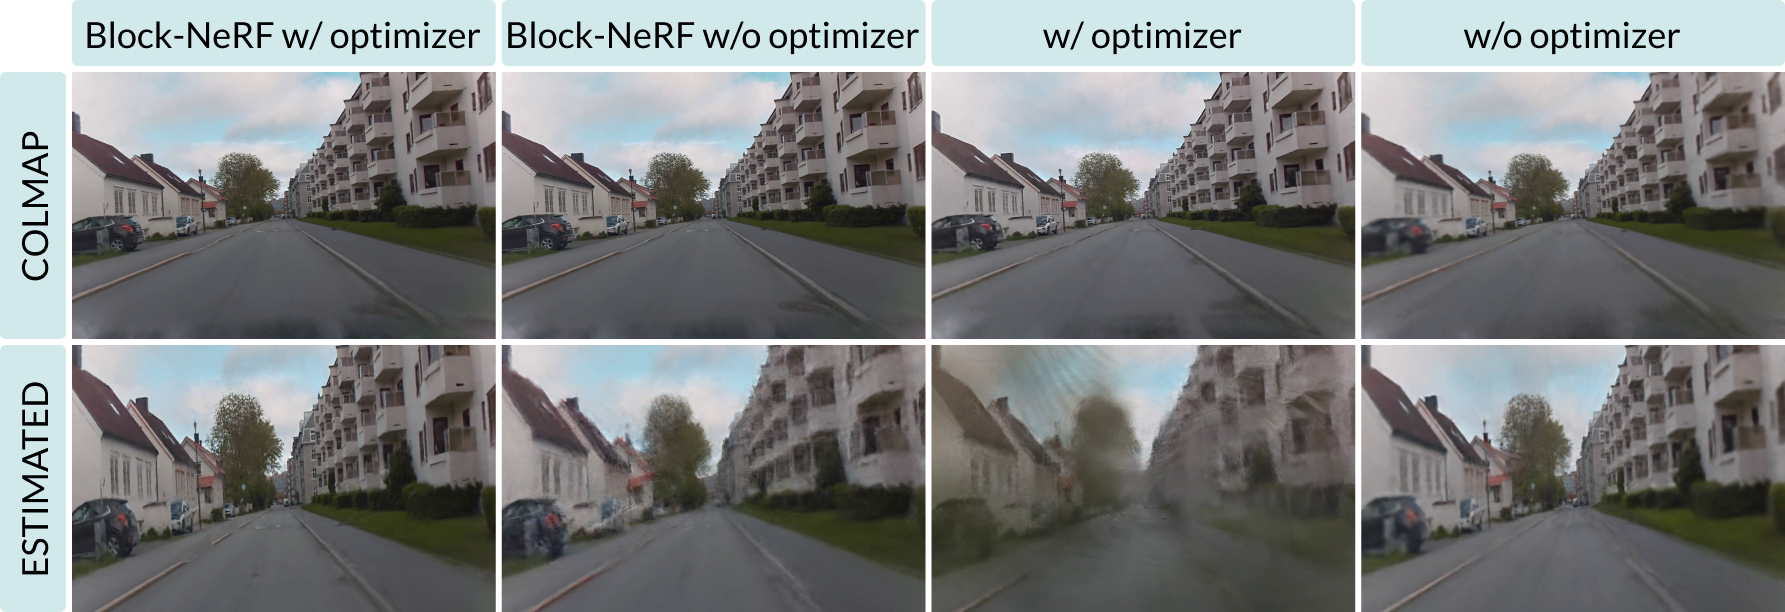
\includegraphics[width=1.0\textwidth]{figures/trip086-comparison.png}
    \caption{Comparison of the different approaches used to train the NeRF on real data. The data is from dataset 1, presented in \autoref{fig:naplab-dataset}.}
    \label{fig:trip086-comparison}
\end{figure}



The results highlight interesting trade-offs between the applied approaches. Notably, the Block-NeRF runs with camera poses approximated by COLMAP without further optimization, yielded the best metrics across all the experiments. Disregarding both Block-NeRF runs, the NeRF trained on images with camera poses approximated with COLMAP and not further optimized yielded the best quantitative results. In contrast, the experiments leveraging \acrshort{gps} readings for camera pose approximations with or without optimization were less successful across all metrics, with the non-optimized \acrshort{gps} approach scoring the lowest across all three metrics.


% Of the runs that don't leverage the naive Block-NeRF approach, the run with camera poses approximated with COLMAP and further optimized camera poses achieves the significantly best PSNR. The COLMAP run without optimizer achieves best SSIM and LPIPS, although the metrics are very similar to the run with optimizer. The qualitative results from the two runs are very different. The run with optimized camera poses appear much more blurry than the one without optimized camera poses.


\begin{comment}
- As expected, the camera optimizer provides better results than the contrary on real data with imperfect camera poses. Atleast it ha a significantly higher PSNR, how do they compare qualitatively?
- As with the synthetic data, the optimized runs appear more blurry, but still achieves better scores on the metrics.


In the set of experiments that did not implement the naive Block-NeRF approach, the results display noteworthy distinctions between different methodologies. The experiment wherein camera poses were approximated using COLMAP and subsequently optimized rendered the highest Peak Signal-to-Noise Ratio (PSNR). This particular experiment demonstrates superior performance in preserving original image detail and quality.

However, interestingly, the experiment utilizing COLMAP without any subsequent optimization yielded the best results in terms of the Structural Similarity Index Measure (SSIM) and the Learned Perceptual Image Patch Similarity (LPIPS). Despite these metrics being extremely close to the COLMAP run with optimization, their distinction in results is worth noting.

Delving deeper into qualitative outcomes, a stark contrast is observed between the two COLMAP runs. The experiment leveraging optimized camera poses generated results with a distinctly higher degree of blurriness compared to its counterpart that did not utilize optimized poses.

This observation highlights the intriguing impact of pose optimization on image clarity and indicates that while certain metrics might be optimized, subjective visual quality and the overall objective might vary significantly. These results collectively underline the complex interplay between technical metrics and perceptual outcomes in the realm of NeRF generation.
\end{comment}


\section{Experiment 6: Novel Views Along Altered Trajectory} \label{sec:altered-trajectories}

An important application of NeRFs is their ability to synthesize high-quality images from novel viewpoints. Although there are many applications for this, one of those is training and evaluating self-driving vehicles. In this section, we will investigate how a NeRF trained on self-captured synthetic and real data can be used to create camera paths and render novel views not previously observed in the dataset. \autoref{fig:altered-trajectories} shows four different camera paths created in Nerfstudio for trained NeRFs.

% In order to investigate how our self-captured data performs for this purpose 
% As previously discussed, NeRF is employed in autonomous vehicle pipelines for this exact purpose.
%This capability could prove particularly useful in applications 
% you need to expand a dataset, e.g. in a machine learning setting, much like you would employ data augmentation.
% One important application of NeRFs is their ability to synthesize images from previously unseen viewpoints, not present in the original dataset. 
% This capability could prove particularly useful in applications where you need to expand a dataset, e.g. in a machine learning setting, much like you would employ data augmentation.


%\begin{figure}[h]
    \centering
    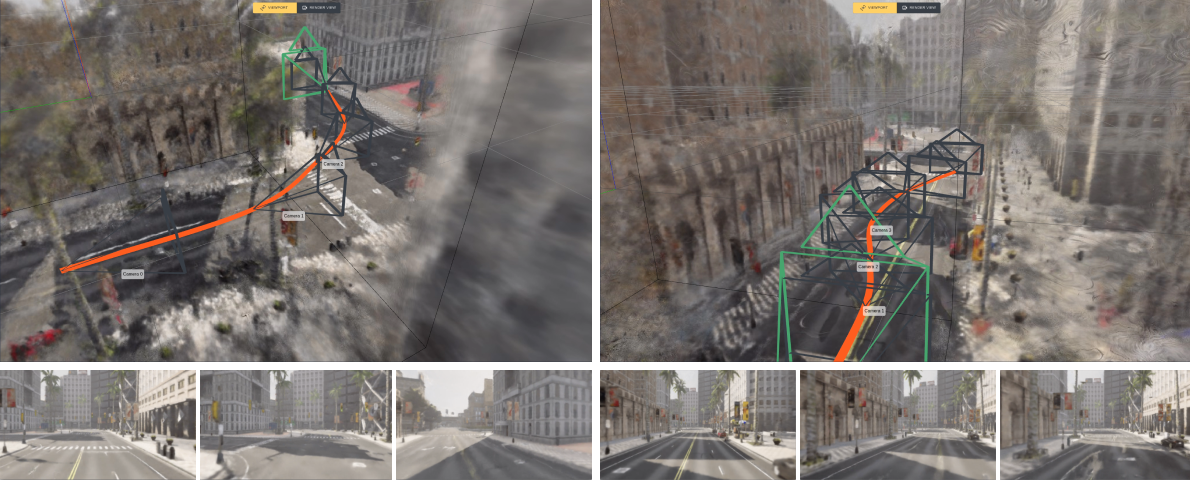
\includegraphics[width=1.0\textwidth]{figures/unseen-trajectories-v2.png}
    \caption{Previously unseen trajectories being rendered by defining a new camera path for the trained NeRF.}
    \label{fig:unseen-trajectories-v2}
\end{figure}
%\begin{figure}[h]
    \centering
    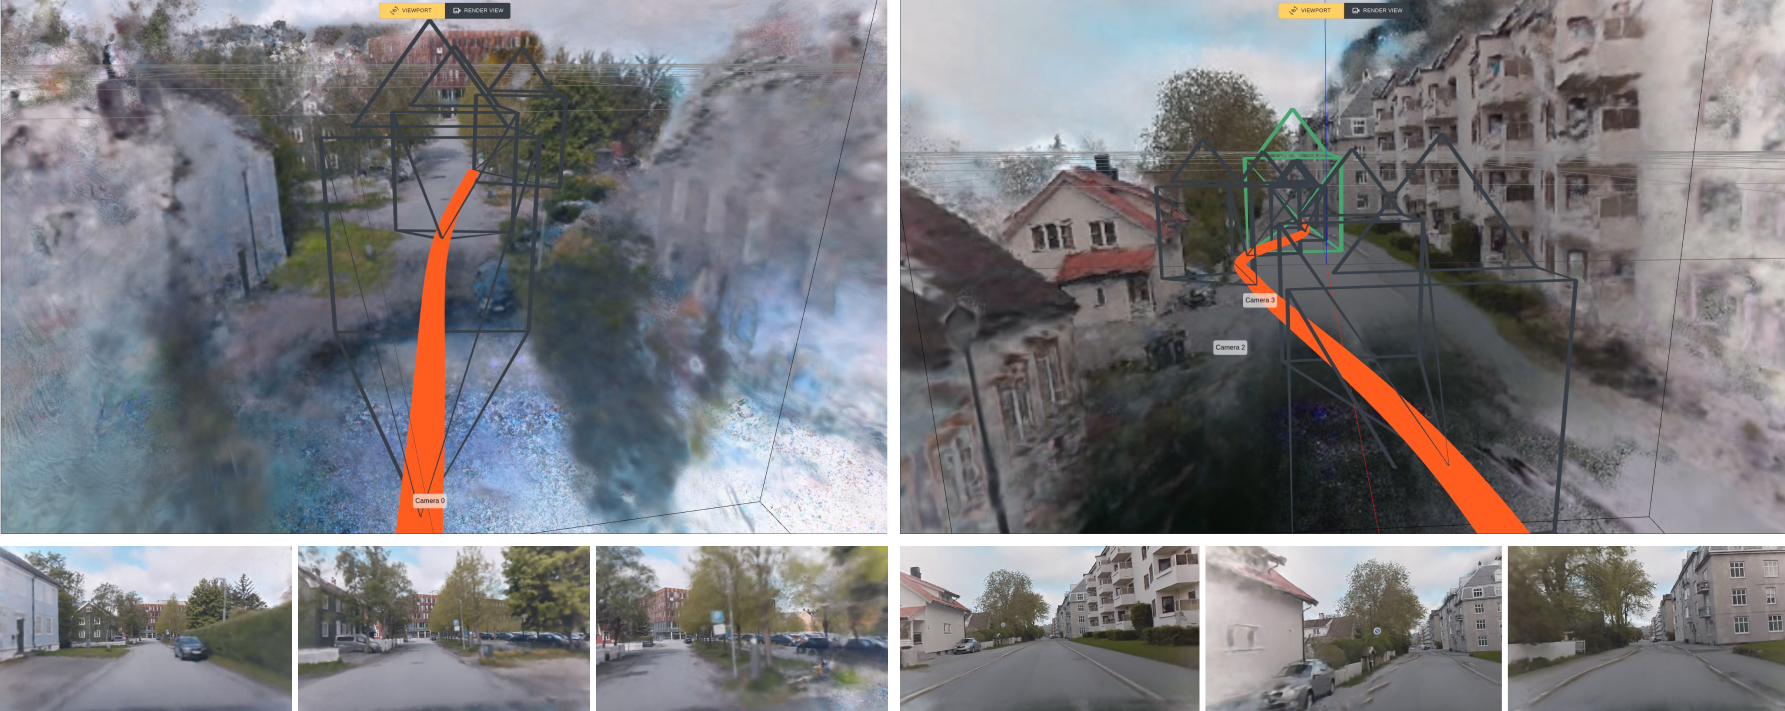
\includegraphics[width=1.0\textwidth]{figures/unseen-trajectories-real-data.png}
    \caption{Previously unseen trajectories being rendered by defining a new camera path for the trained NeRF. Left) From dataset 3 with a trajectory into a road sign, right) from dataset 1 with a swerving trajectory across the curb.}
    \label{fig:unseen-trajectories-real-data}
\end{figure}
\begin{figure}[h]
    \centering
    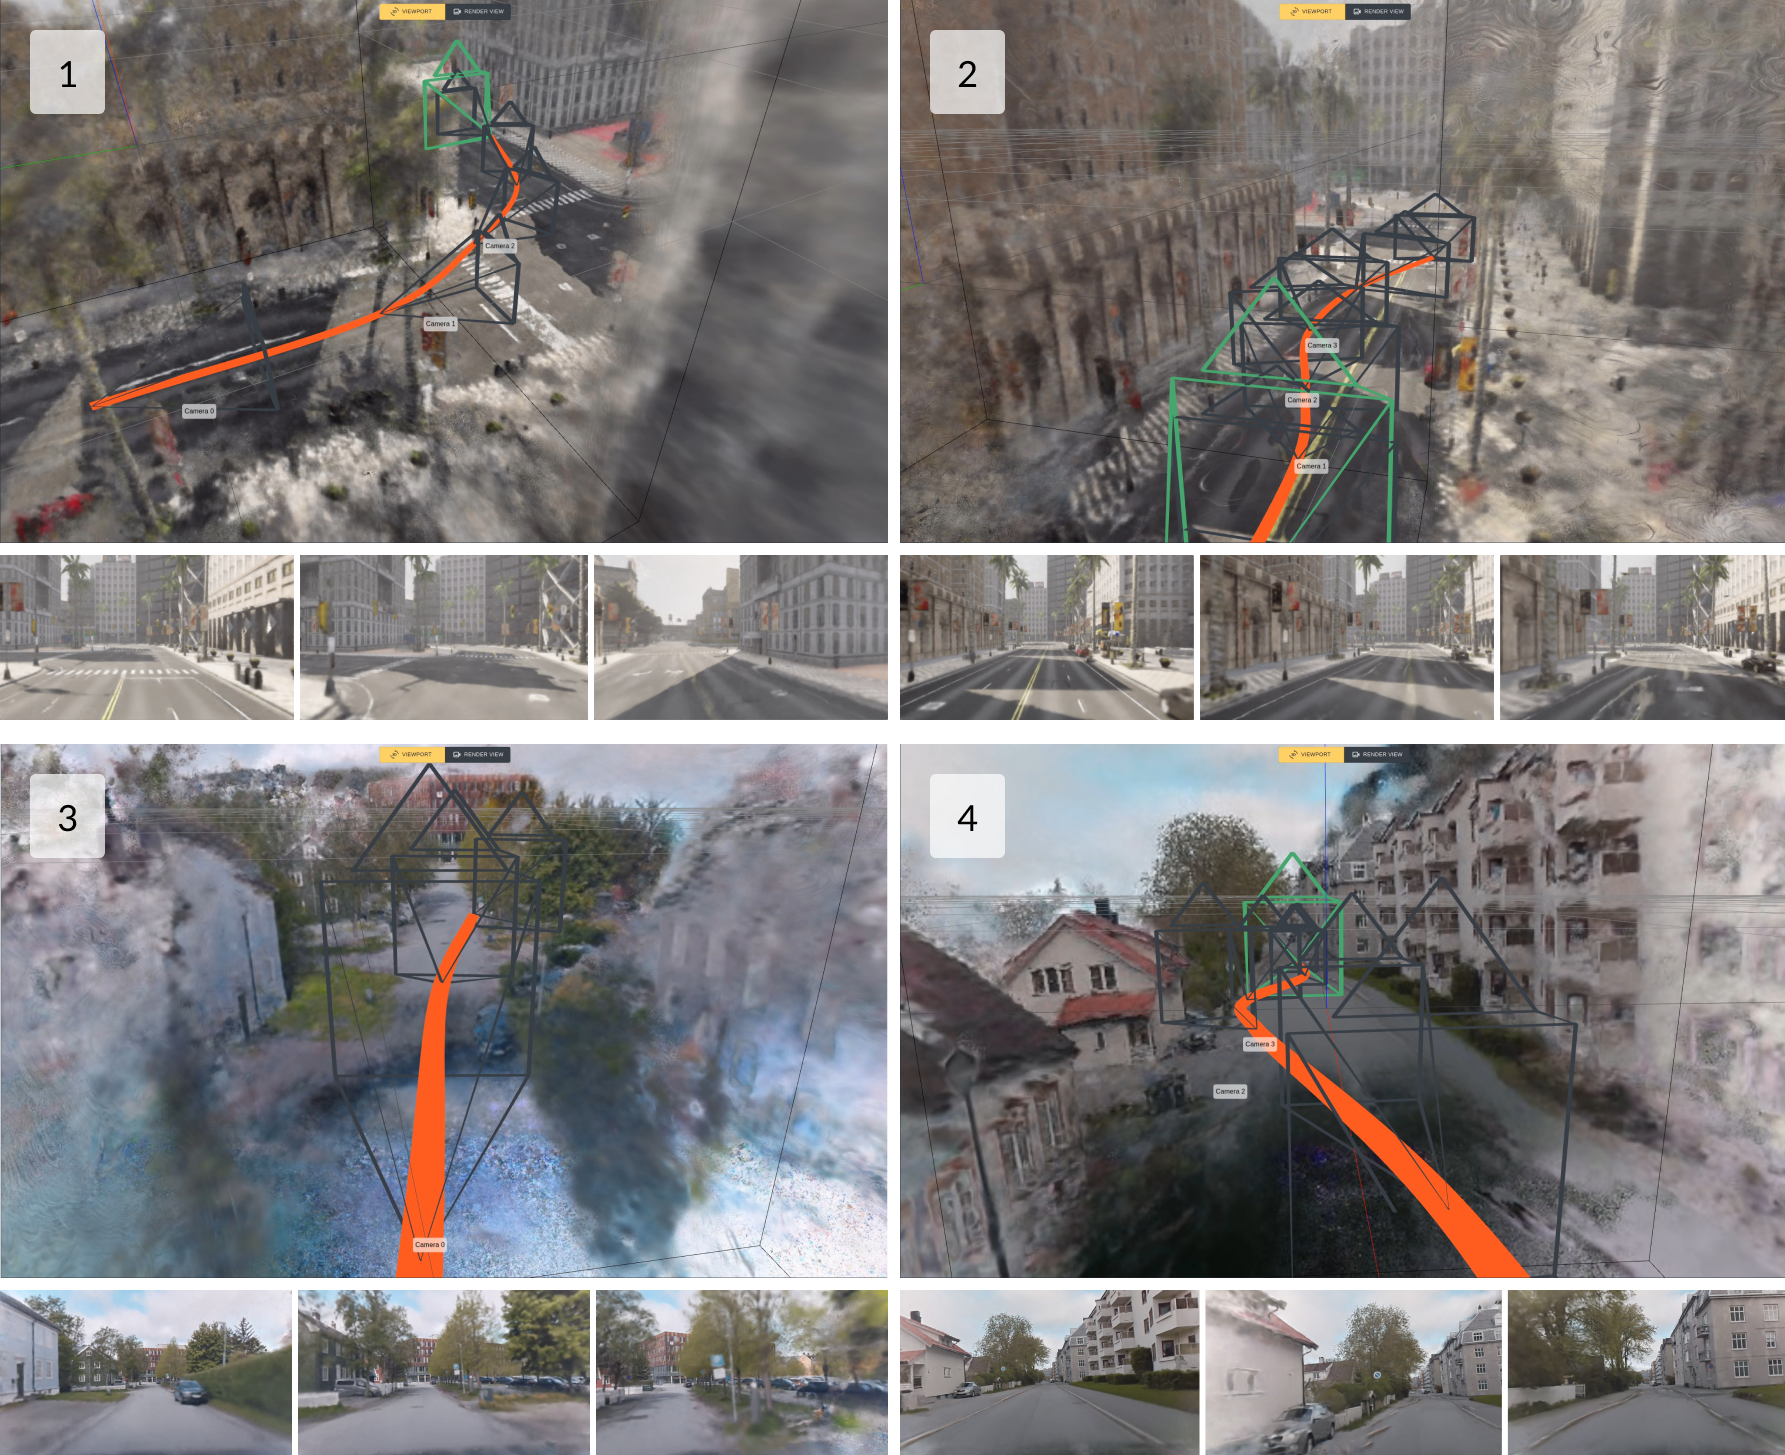
\includegraphics[width=1.0\textwidth]{figures/altered-trajectories.png}
    \caption[Results from experiment 6: Altered trajectories]{Previously unseen trajectories being rendered by defining a new camera path for the trained NeRF. Image 1 illustrates a trajectory deviating across a traffic light zone, while image 2 shows a trajectory veering into the opposing lane. Image 3, derived from dataset 3, portrays a trajectory directed towards a road sign, and Image 4, derived from dataset 1, presents a trajectory swerving over the curb. The \acrshort{naplab} datasets are presented in \autoref{fig:naplab-dataset}.}
    \label{fig:altered-trajectories}
\end{figure}




% For discussion
% The scene has only been seen from a very limited number of views. In order to generate high-quality novel views, the same scene should be observed from multiple viewpoints.